%~~~~~~~~ Chapter ~~~~~~~~
\chapter{Graphene}
\label{ch:graphene}

%
% TODO
% - Comparison bands 4 orbital 1 orbital
% - Dirac description?
%
%2) Background chapter (90%)
%   - TB 1 orbital
%  - TB 4 orbitales
%   - SOC (origin in 4 orbital model)   Connection between the 2D graphene with SOC and 4 orbitals,  the  gap= sublattice* spin*valley,  the Kane & Mele model  for G. Monolayer.
%   -  Graphene monolayer + Bilayer
%   - Topological phases (Z2, edge states, Kane Mele model)


Graphene is one of the most studied materials in history\cite{KatsnelsonBook, Geim2007, Murakami2009, CastroNeto2009a,
Mas-Balleste2011, Konschuh2011a, Cooper2012, Han2014, Sadurni2014, Rozhkov2016}.
Even before its experimental discovery\cite{Novoselov2004, Novoselov2005},
extensive research was devoted to it\cite{Wallace1947, VanBommel1975, Semenoff1984, Haldane1988, Forbeaux1998, Oshima2000}.
All the basic properties have been discussed profusely, yet, for the sake of completeness I will make a brief recap of all the properties relevant for the rest of this thesis.\\

Graphene consists of a two-dimensional array of carbon, $C$, atoms arranged in a honeycomb structure\cite{Huang2011} % TODO more references
like the one shown in \fref{graphene_summary}(a,b) % ~$a,b)$.
Unless otherwise stated, we will consider that the unstrained atomic distance between carbon atoms is $d_{C-C}=a=\SI{1.4}{\angstrom}$ in accordance with literature\cite{KatsnelsonBook, Cooper2012, Ishigami2007}. % TODO more biblio

%~~~~~~~~~~~~~~~~~~~~~~~~~~ FIGURE ~~~~~~~~~~~~~~~~~~~~~~~~~%
\begin{figure}[h!]
\centering
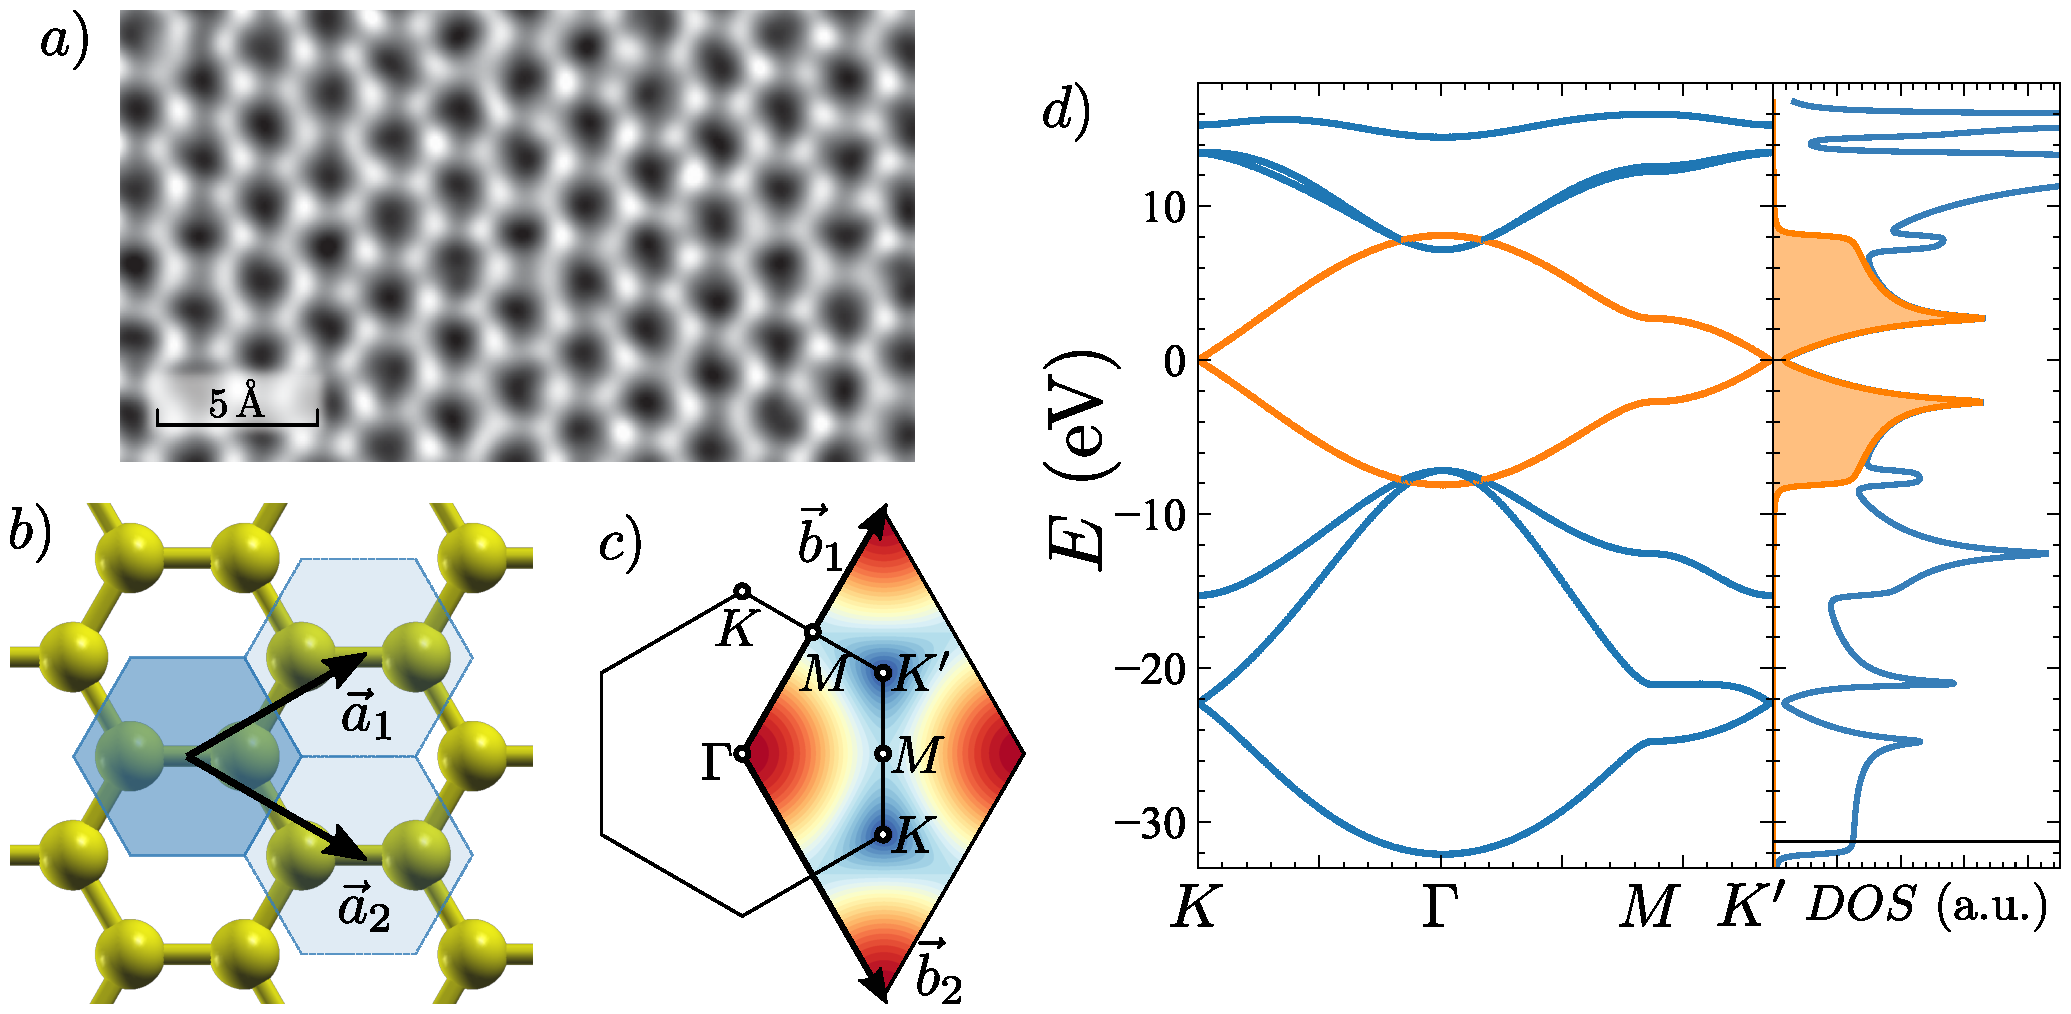
\includegraphics{graphene/figures/graphene_summary.pdf}
\vspace{-5pt}
\caption{$a)$ STM image of graphene taken from ref~\cite{Huang2011}. $b)$ Cartoon depiction of the atomic structure of graphene using the lattice vectors defined in \eqref{latt_vec}. $c)$ Reciprocal vectors $\vec{b}_i$ and two representations of the \acf{fbz}. $c)$ Band structure of graphene calculated in the tight-binding approximation (details later in the text).}
\label{graphene_summary}
\end{figure}
\FloatBarrier
%~~~~~~~~~~~~~~~~~~~~~~~~~~~~~~~~~~~~~~~~~~~~~~~~~~~~~~~~~~~%

The honeycomb structure is not a Bravais lattice, so, in order to describe the system in terms of Bloch functions, we have to choose a unit cell and the appropriate lattice vectors to tessellate the space.
Naturally there are infinite possibilities to do so, but the simplest one is that depicted in \fref{graphene_summary}b).
The simplest unit cell and  Bravais lattice with which we can describe graphene is the one depicted in \fref{graphene_summary}a). It consists of two atoms in the positions
\begin{equation}
\vec{r}_0 = \tfrac{a}{2}(-1,0,0) \quad;\quad
\vec{r}_1 = \tfrac{a}{2}(1,0,0),
\label{at_pos}
\end{equation}
The lattice vectors that define the triangular Bravais lattice are:
\begin{equation}
\vec{a}_1 = \tfrac{a}{2}\left(3,\sqrt{3},0\right) \quad;\quad
\vec{a}_2 = \tfrac{a}{2}\left(3,-\sqrt{3},0\right)
\label{latt_vec}
\end{equation}
This geometry defines a hexagonal Wigner-Seitz cell (blue region on \fref{graphene_summary}b)) with area $\sim\SI{5.1}{\angstrom\squared}$.

The reciprocal lattice vectors are depicted in \fref{graphene_summary}c) and can be easily calculated using the relation: $\vec{a}_i\vec{b}_j=2\pi\delta_{ij}$. Notice that the canonical \ac{fbz} shown in \fref{graphene_summary}c) is an hexagon (just like the Wigner–Seitz cell) but nothing changes if instead we use the gray shadowed region, which is much more convenient for computational calculations.\\


Once the lattice structure is clear, we turn to the electronic properties. Carbon atoms have 6 electrons allocated in five orbitals distributed in the layers with quantum number $n\in\{1,2\}$.
The first two electrons are in the $1s$ level, two more in the $2s$ level and finally another two \acp{el} in the $2p$ levels (\fref{orbitals}).
%~~~~~~~~~~~~~~~~~~~~~~~~~~ FIGURE ~~~~~~~~~~~~~~~~~~~~~~~~~%
\begin{figure}[h!]
\centering
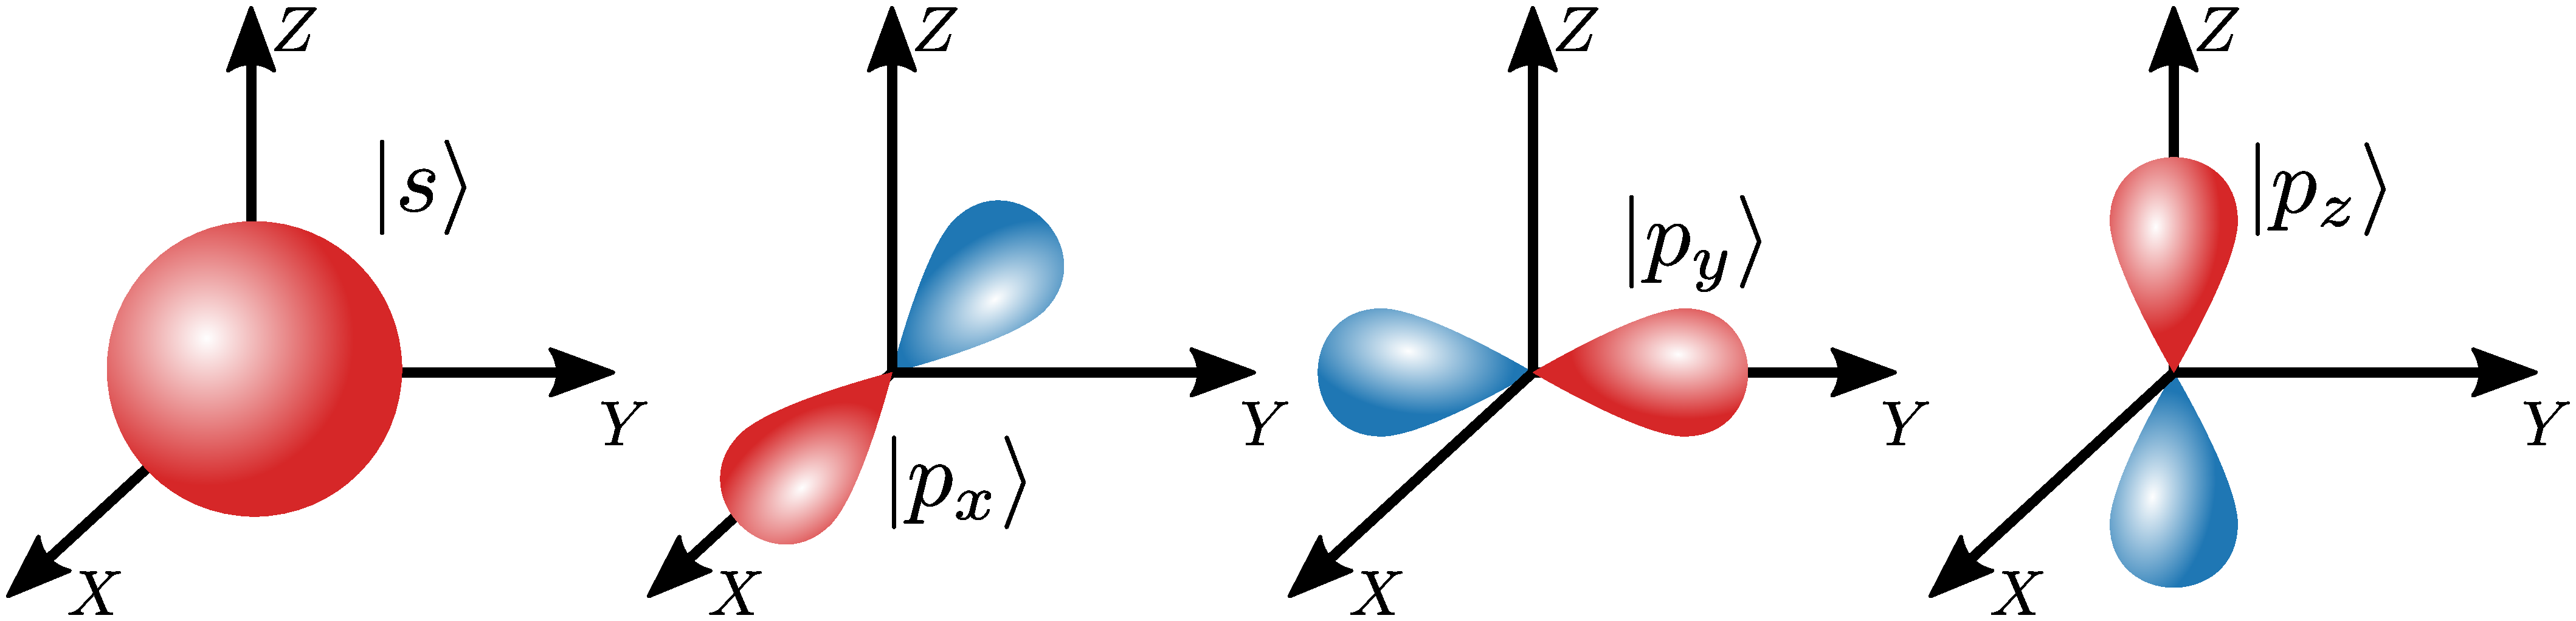
\includegraphics{graphene/figures/orbitals.pdf}
\vspace{-5pt}
\caption{Cartoon depiction of the hydrogenoid orbitals involved in the graphene chemical and physical properties. The color of the orbitals shows the parity of the orbital what will be relevant when building tight-binding models.}
\label{orbitals}
\end{figure}
\FloatBarrier
%~~~~~~~~~~~~~~~~~~~~~~~~~~~~~~~~~~~~~~~~~~~~~~~~~~~~~~~~~~~%
Since the orbitals $n=1$ are doubly occupied and far down in energy, there is no need to consider them. The $2s$ level is also full, but they show a strong hopping with the $p$ orbitals which are around the Fermi energy so we will consider their contribution. The $2p$ orbitals are the closest to the Fermi level, hence they will play a major role in the chemistry of graphene.\\

With this description of the system we can build a basis which will have four orbitals per Carbon atom:
\begin{equation}
  \mathcal{B}_4 = \left\{
  \ket{\phi^1_{s}},\ket{\phi^1_{p_x}},\ket{\phi^1_{p_y}},\ket{\phi^1_{p_z}},
  \dots,
  \ket{\phi^n_{s}},\ket{\phi^n_{p_x}},\ket{\phi^n_{p_y}},\ket{\phi^n_{p_z}}
  \right\}
\label{basis4}
\end{equation}
where the superscript points out the atom and the subscript shows the corresponding orbital. The bands resulting from this description are shown in \fref{graphene_summary}d). We will delve in the physical properties later on, but for now it should suffice to point out the linear dispersion in the $K$ and $K'$ points around the Fermi energy $E_F=\SI{0}{\eV}$ as well as the decoupling of the two bands (from the $p_z$ manifold) colored in orange. The \ac{dos} show that the orbitals involved only have weight in those two bands as we will see later.

In many cases we will not be interested in the properties of the orbitals that do not contribute to those two bands. In those cases we will reduce our basis and consider only one orbital per Carbon atom, resulting in the basis:
\begin{equation}
  \mathcal{B}_1 = \left\{\ket{\phi^1_{p_z}}, \ket{\phi^2_{p_z}},\dots, \ket{\phi^n_{p_z}}\right\}
\label{basis1}
\end{equation}

In the next section we show the details of the model used to build the Hamiltonians used all along this thesis.


\section{Slater-Koster tight-binding model}
\label{ssec:SK}
Generally the hopping parameters are an input in any \ac{tb} model. They are usually calculated by fitting eigenvalues (and possibly eigenfunctions) obtained from \ac{dft} calculations. Another way to calculate the hopping parameters is to project the eigenfunctions into a basis of localized atomic orbitals so the interpretation in terms of hydrogenoid orbitals is easier.

As a system grows complex, more and more parameters are needed to describe it. In fact, the number of hoppings grows with the size of the basis, $n_\mathcal{B}$, as $\sum^{n_\mathcal{B}}_i i$. Nevertheless since the number of different orbitals is finite and a larger basis means only a more complex arrangement of orbitals, one could expect that not every parameter is completely independent from the others.
%~~~~~~~~~~~~~~~~~~~~~~~~~~ FIGURE ~~~~~~~~~~~~~~~~~~~~~~~~~%
\begin{figure}[h!]
\centering
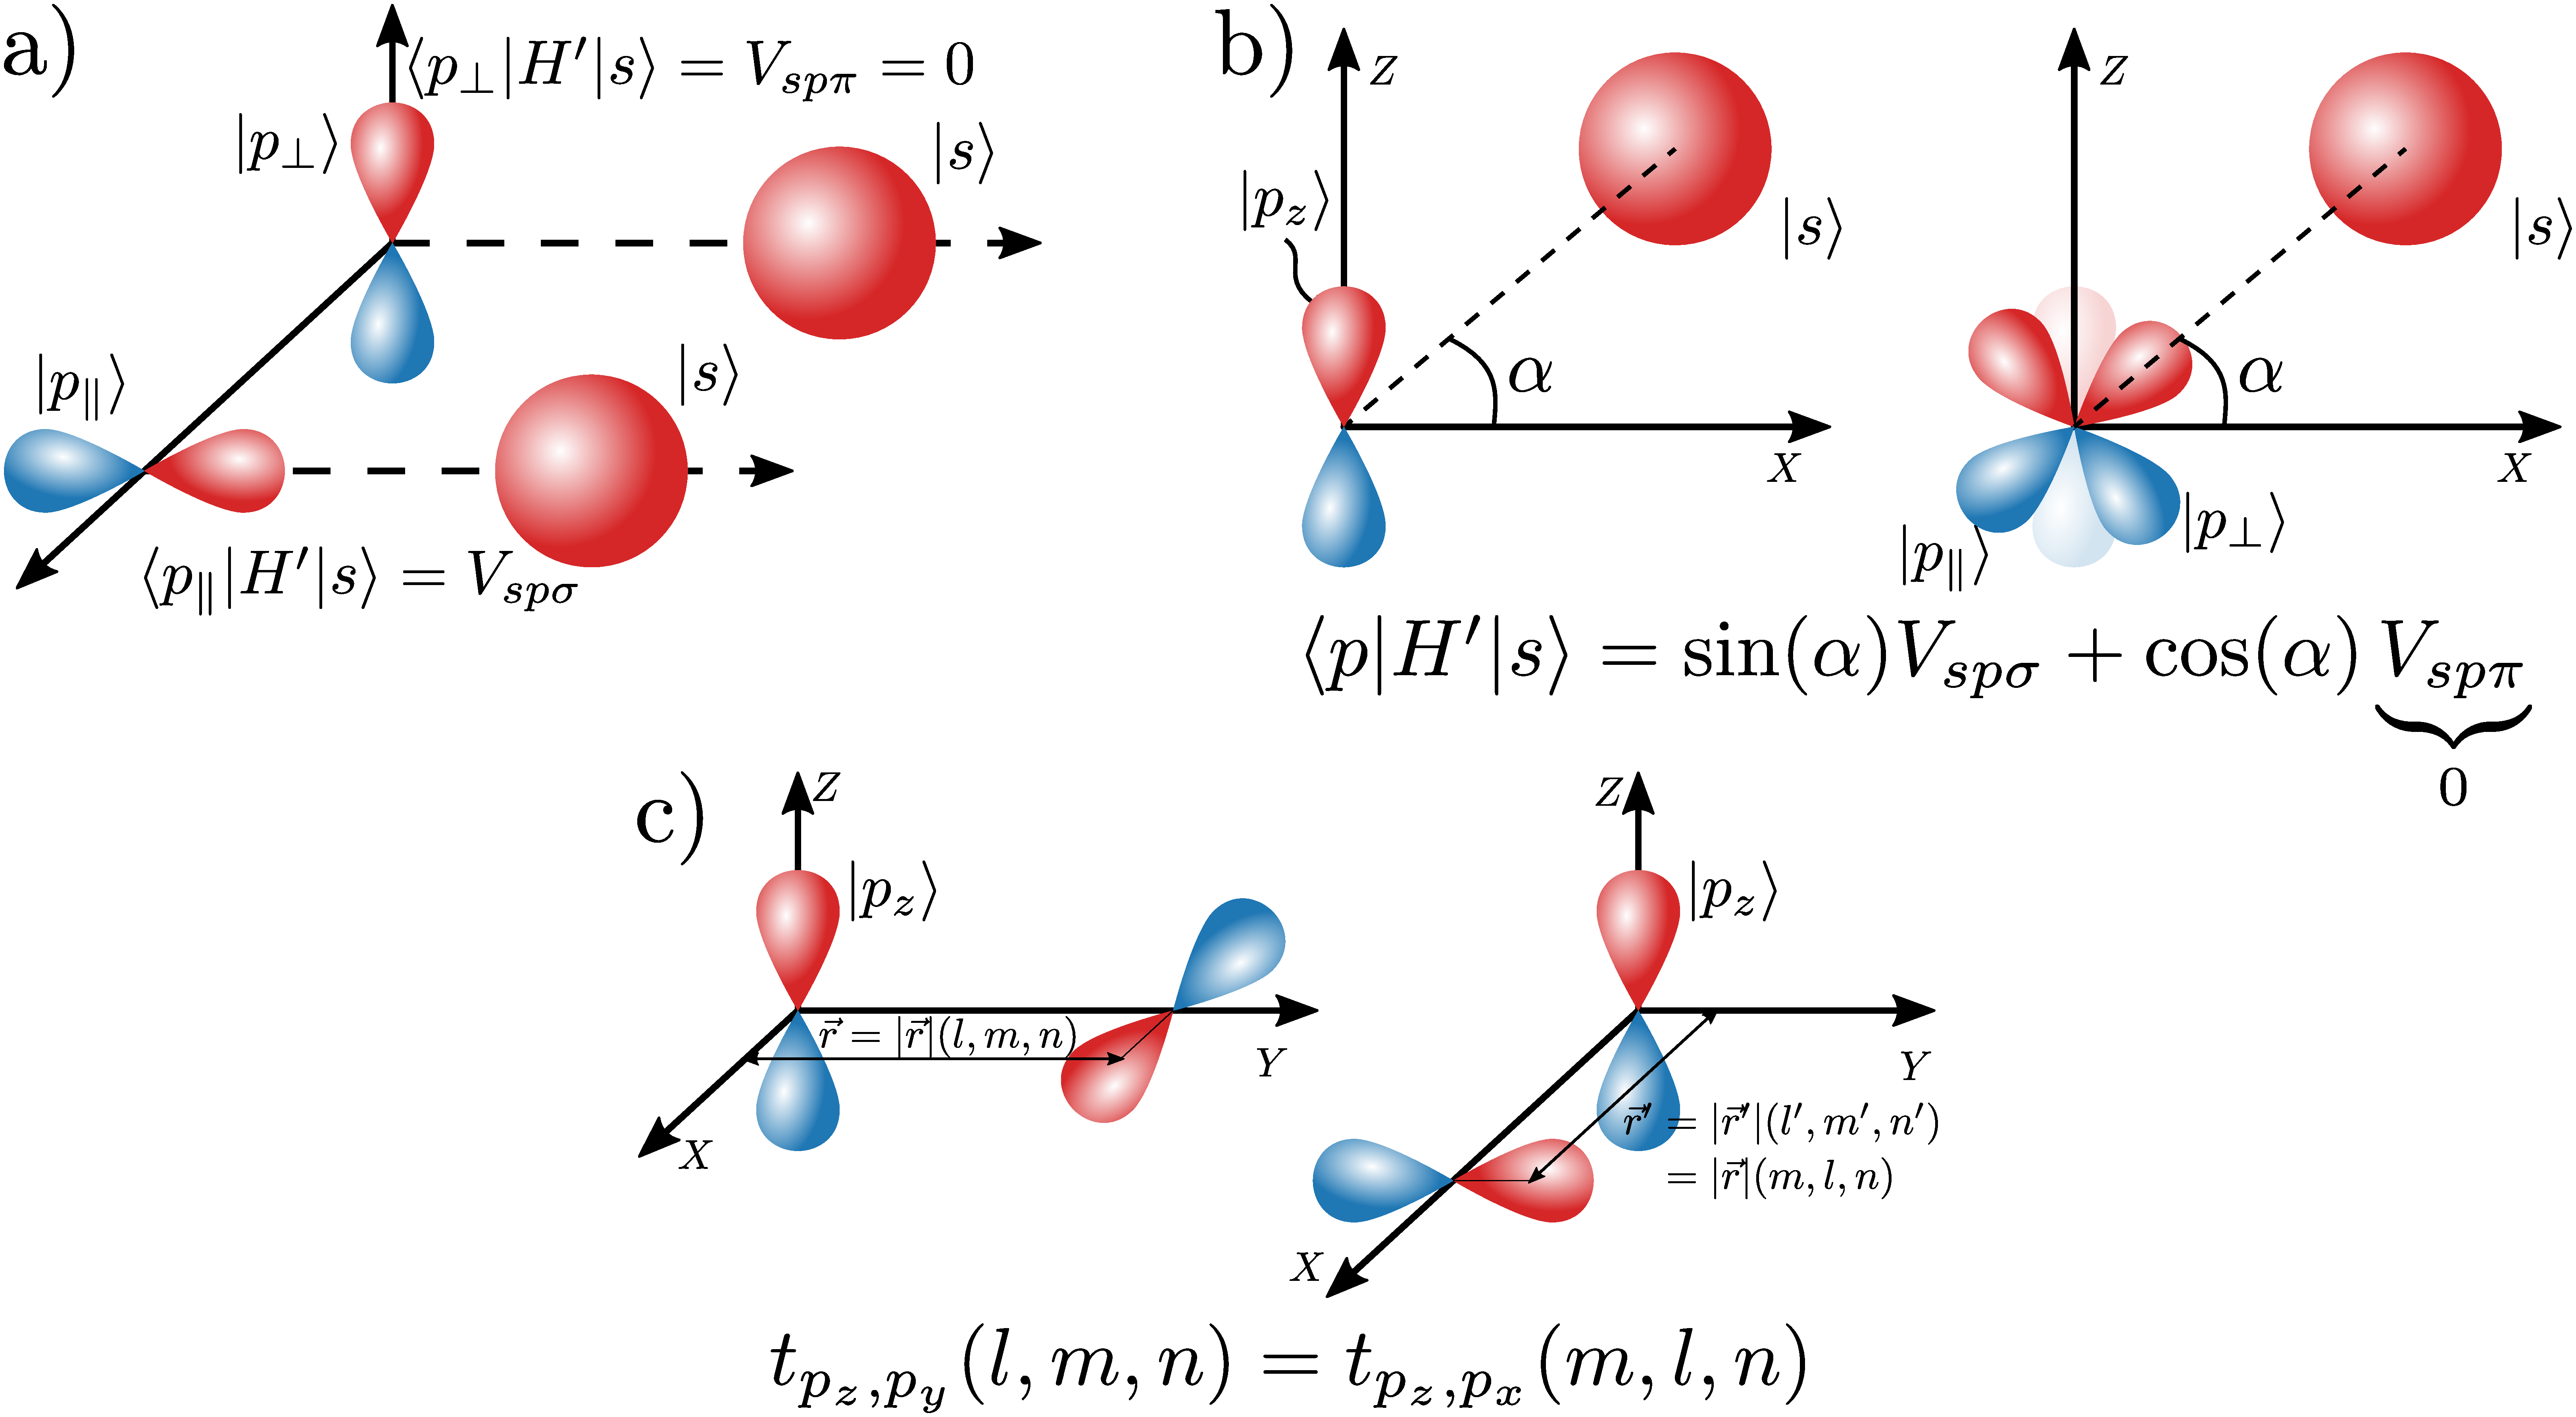
\includegraphics{graphene/figures/hoppings.pdf}
\vspace{-10pt}
\caption{$a)$ Definition of the parallel and perpendicular hoppings. Notice that $V_{sp\pi}=0$ because of the symmetry of the orbitals. $b)$ Decomposition of a $p_z$-$s$ hopping in terms of its parallel and perpendicular projections. $c)$ Using the symmetry of the orbitals we can relate different hopping integral by simple rotations.}
\label{fig:SK}
\end{figure}
\FloatBarrier
%~~~~~~~~~~~~~~~~~~~~~~~~~~~~~~~~~~~~~~~~~~~~~~~~~~~~~~~~~~~%
The \ac{sk} approximation\cite{Slater1954} takes into account the symmetry of the atomic orbitals to reduce the number of parameters needed since some of them are related by rotations or other symmetry operations.

The \ac{sk} model encodes the two-center hopping integrals $t_{\phi_1-\phi_2} = \bra{\phi_1(\vec{r})}H'(\vec{r},\vec{r}')\ket{\phi_2(\vec{r'})}$ along high symmetry directions in a set of constants: $V_{\alpha\alpha'm}$, where $\alpha$ and $\alpha'$ label the orbitals and m refer to the component of angular momentum around the line between the center of the two orbitals. In \fref{fig:SK}a) it can be seen how the $V_{sp\pi}$ and $V_{sp\sigma}$ are defined\footnote{Notice that $V_{sp\pi}$ automatically vanishes because of the symmetry of the orbitals.}
It is important to notice that the radial information is enclosed in the \ac{sk} parameters. In general the \ac{sk} parameters will decrease as the distance between the orbitals increases, the exact ratio depends on the orbitals and different approximations can be found in the literature.\cite{Harrison1930}\\


By decomposing the hopping integrals in parallel and perpendicular components we reduce the number of parameters needed to account for all possible hoppings. For instance, we only need two parameters: $V_{pp\sigma}$ and $V_{pp\pi}$ in order to express all six $p-p$ hoppings.

This description of the hopping parameters also accounts for the symmetry of the orbitals. For instance \fref{fig:SK}c) it is shown the relation between the hoppings $t_{p_{z},p_{x}}$ and $t_{p_{z},p_{y}}$. If we forget about the labels in the axis, we can realize that these two hoppings are in fact equivalent since one can be obtained as a rotation of the other.

If we define the unitary vector $\hat{r} = \vec{r}/|\vec{r}|$ and its components $\hat{r}=(l,m,n)$ we can see that
\begin{equation}
  t_{p_{z},p_{x}} (l,m,n) = t_{p_{z},p_{y}}(m,l,n)
\end{equation}
notice that the change in the arguments is equivalent to perform a rotation of the vector $\vec{r}$ of $-\pi/2$ around the $Z$ axis.\\

The \ac{sk} description of the \ac{tb} hopping integrals allows the formulation of all the hoppings in terms of a few parameters which encode the distance between orbitals at the same time that it preserves the angular information in the analytical formulation which can be checked in appendix \ref{SKhoppings}.


\subsection{Slater-Koster versatility}
\subsubsection{Angular dependence}
An example of this decoupling can be shown in the following gedankenexperiment. Let us consider graphene and let us displace vertically a little bit one of the sublattices\footnote{If it boggles your mind you can shift all the atomic positions to keep the $C$-$C$ distance as $a=\SI{1.4}{\angstrom}$}
so we end up with a slightly distorted graphene in which not all the atoms are in the same plane. This shift out of the plane has an important effect in the band structure since it breaks the mirror symmetry that kept the $p_z$ orbitals isolated from every other orbital.
This mixing of the $p_z$ manifold with all the other orbitals happens mainly at $\Gamma$ and it can be seen in both in the band structure and in the \ac{dos}
%~~~~~~~~~~~~~~~~~~~~~~~~~~ FIGURE ~~~~~~~~~~~~~~~~~~~~~~~~~%
\begin{figure}[h!]
\centering
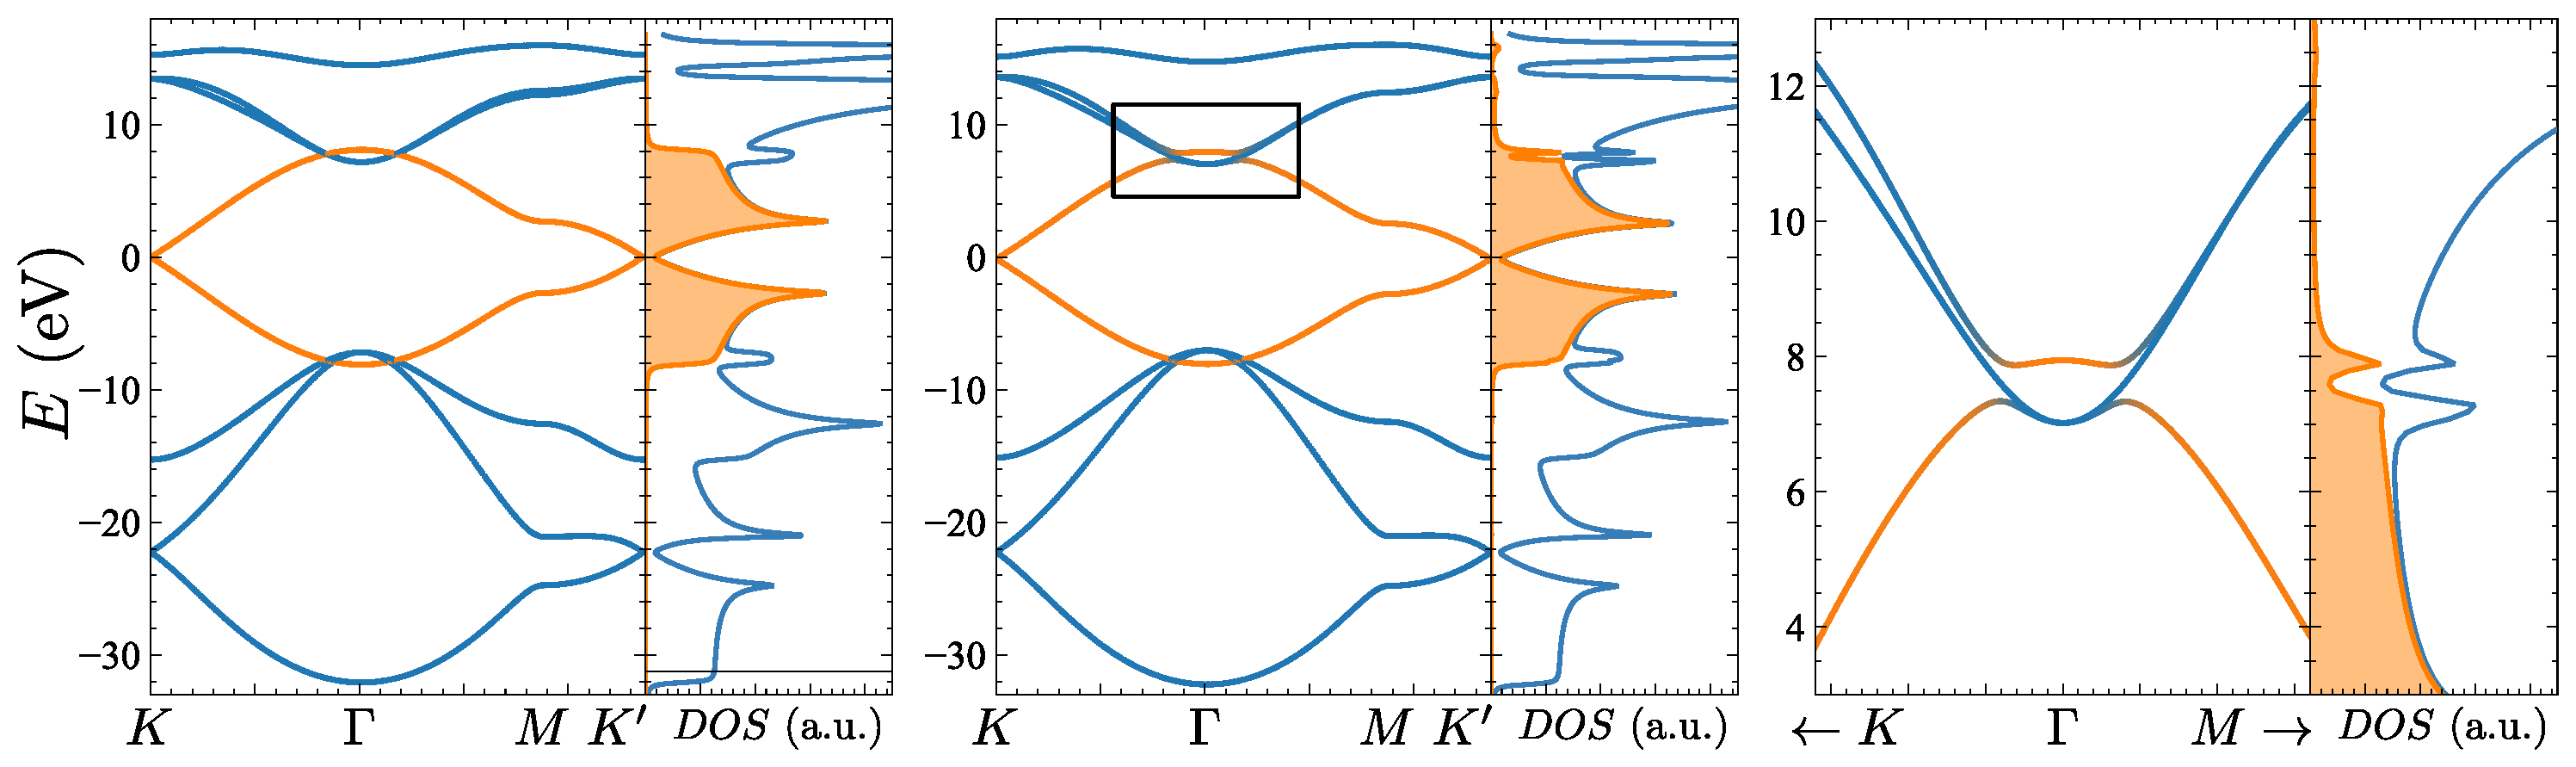
\includegraphics{graphene/figures/banddos_G_buck.pdf}
\vspace{-5pt}
\caption{a) Pristine graphene band structure and DOS. b) Buckled graphene band structure and DOS. c) zoom around the $\Gamma$ point where the $\sigma$-orbitals hybridize with the $\pi$-manifold.}
\label{fig:buckling}
\end{figure}
\FloatBarrier
%~~~~~~~~~~~~~~~~~~~~~~~~~~~~~~~~~~~~~~~~~~~~~~~~~~~~~~~~~~~%
This simple example shows how easy it is to account for geometric distortions. The buckling used in this example is similar to that naturally occurring in other materials such as 2-D Bismuth crystals.

\subsubsection{Other materials}
Once we have the machinery to build \ac{sk} hamiltonians, simply by changing the \ac{sk} parameters we can describe different materials.
In this section we compare graphene, bismuth and $h-BN$  % TODO cite
as simple examples where the \ac{sk} description works well.\\

%
% Graphene TB
%
In order to describe graphene, different sets of parameters can be found in the literature\cite{}. Nevertheless some of the parameters used here have been fitted from \ac{dft} calculations. The \ac{sk} parameters in $\si{\eV}$ used for graphene are:
\begin{equation}
  \begin{array}{l|cccc}
    Hopping & V_{ss\sigma} & V_{sp\sigma} & V_{pp\sigma} & V_{pp\pi} \\ \hline
    C-C & -7.76 & 8.16 & 7.48 & -2.7 \\
    C-H & -6.84 & 7.81 & \text{--} & \text{--}
  \end{array}\qquad\qquad
  \begin{array}{c|cccc}
    \text{On-site} & s & p_x & p_y & p_z \\ \hline
    C & -8.8 & 0.0 & 0.0 & 0.0 \\
    H & -2.5 &     &     &
  \end{array}
\label{G_SK_params}
\end{equation}
where the hoppings with a hypothetical $H$ atom have been included for later convenience.\\

To describe the relevant features of $h-BN$ it suffices to add a different on-site energy for the $B$ and $N$ ($E_{B} = -E_{N} =\SI{2.5}{\eV}$) atoms while keeping the inter-atomic hoppings similar to those of graphene.\\

Bismuth is a little bit more complex since an accurate description requires up to third neighbor hoppings (and spin-orbit coupling as well, which we will neglect for the moment). The \ac{sk} parameters, taken from~\citen{Liu1995} are:
\begin{equation}
  \begin{array}{c|cccc}
    Hopping & V_{ss\sigma} & V_{sp\sigma} & V_{pp\sigma} & V_{pp\pi} \\ \hline
    1 & -0.608 & 1.32 & 1.854 & -0.6 \\
    2 & -0.384 & 0.433 & 1.396 & -0.344 \\
    3 & \text{--} & \text{--} & 0.156 & \text{--}
  \end{array}\quad\qquad
  \begin{array}{c|cc}
     \text{On-site} & s & p_{x,y,z} \\ \hline
    Bi & -10.906 & -0.486
  \end{array}
\label{Bi_SK_params}
\end{equation}\\

The respective band structure of all these materials is shown in \fref{SKbands}.
For all panels, the color, $\mathcal{C}$ represents the weight of the $p_z$ orbital in each state:
\begin{equation*}
   \mathcal{C} = \bra{\psi_{\alpha}}\mathcal{O}_{p_z}\ket{\psi_{\alpha}}
\end{equation*}
where $\mathcal{O}_{p_z}$ is the $p_z$ projector operator and $\ket{\psi_{\alpha}}$ are the Hamiltonian eigenfunctions.
\begin{equation*}
  H\ket{\psi_{\alpha}} = E_{\alpha}\ket{\psi_{\alpha}} \qquad ; \qquad
   \ket{\psi} = \sum_i c_i\ket{\phi_i} \quad
   \text{for} \quad\ket{\phi_i}\in\mathcal{B}_4
\end{equation*}
%~~~~~~~~~~~~~~~~~~~~~~~~~~ FIGURE ~~~~~~~~~~~~~~~~~~~~~~~~~%
\begin{figure}[h!]
\centering
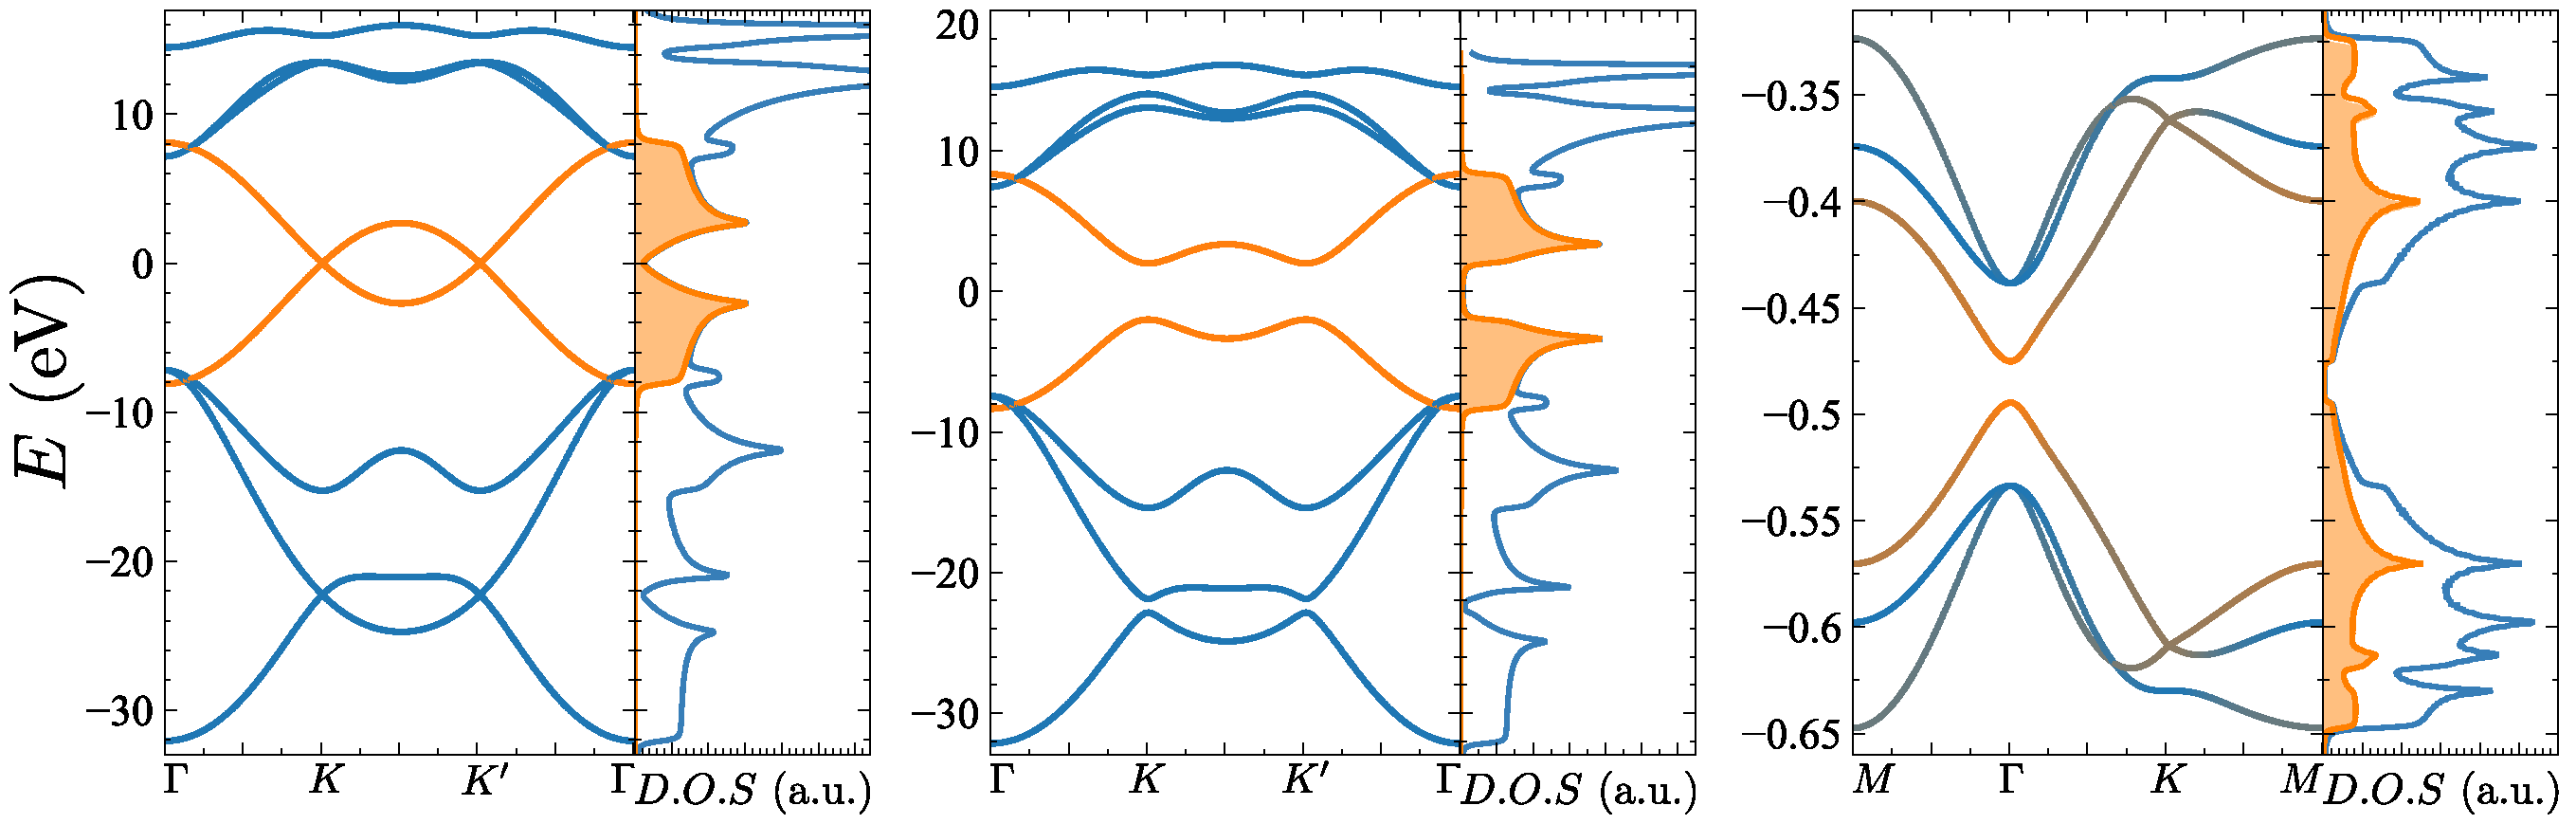
\includegraphics{graphene/figures/banddos.pdf}
\vspace{-15pt}
\caption{a) Graphene bands in the \ac{sk} approximation, with $s$, $p_x$, $p_y$, $p_z$ orbitals for the $C$ atoms. The color denote the $p_z$ component of each state. It can be seen that the $p_z$ orbital are decoupled from the rest of the orbitals. b) $h-BN$ band structure, similar to that of graphene, but with a gap open due to the difference in the on-site energies between the $B$ and $N$ atoms. c) Bismuth band structure, since its atomic structure is buckled, the $p_z$ orbital is not decoupled from the others as it can be seen by the smooth change in color of the central bands.}
\label{SKbands}
\end{figure}
\FloatBarrier
%~~~~~~~~~~~~~~~~~~~~~~~~~~~~~~~~~~~~~~~~~~~~~~~~~~~~~~~~~~~%


\section{Basic Properties}
\label{sec:graphene_basic_properties}
%
%  General description of bands
%  Low energy,
%
We are going to use a \ac{tb} model in the \ac{sk} approximation with four orbitals per carbon atom to describe graphene. The band structure obtained with this model is shown in \fref{bandsG}.

The first thing to notice about the graphene bands is the orbital distribution of the bands. As mentioned before the $p_z$ orbitals are responsible for the central bands, crossing the Fermi energy at $E_F=\SI{0.0}{\eV}$. Due to the mirror symmetry (with respect to the atomic plane), every hopping between the $\sigma$-orbitals and $p_z$ vanishes exactly (see the definition of $V_{sp\sigma}$ in \fref{orbitals}a)).
The presence of \textit{only} $p_z$ orbitals around the Fermi energy makes it possible to describe the system solely with these orbitals.

The second thing to notice is that around the Fermi level, the band dispersion is linear. In particular, the band structure forms two pairs of cones in the $K$ and $K'$ points of the \ac{fbz}. This famous feature %TODO cite
%is responsible for many of the interesting properties of graphene %TODO cite{Klein, HEP analogies, anomalies, topology,...}
%~~~~~~~~~~~~~~~~~~~~~~~~~~ FIGURE ~~~~~~~~~~~~~~~~~~~~~~~~~%
\begin{figure}[h!]
\begin{center}
  %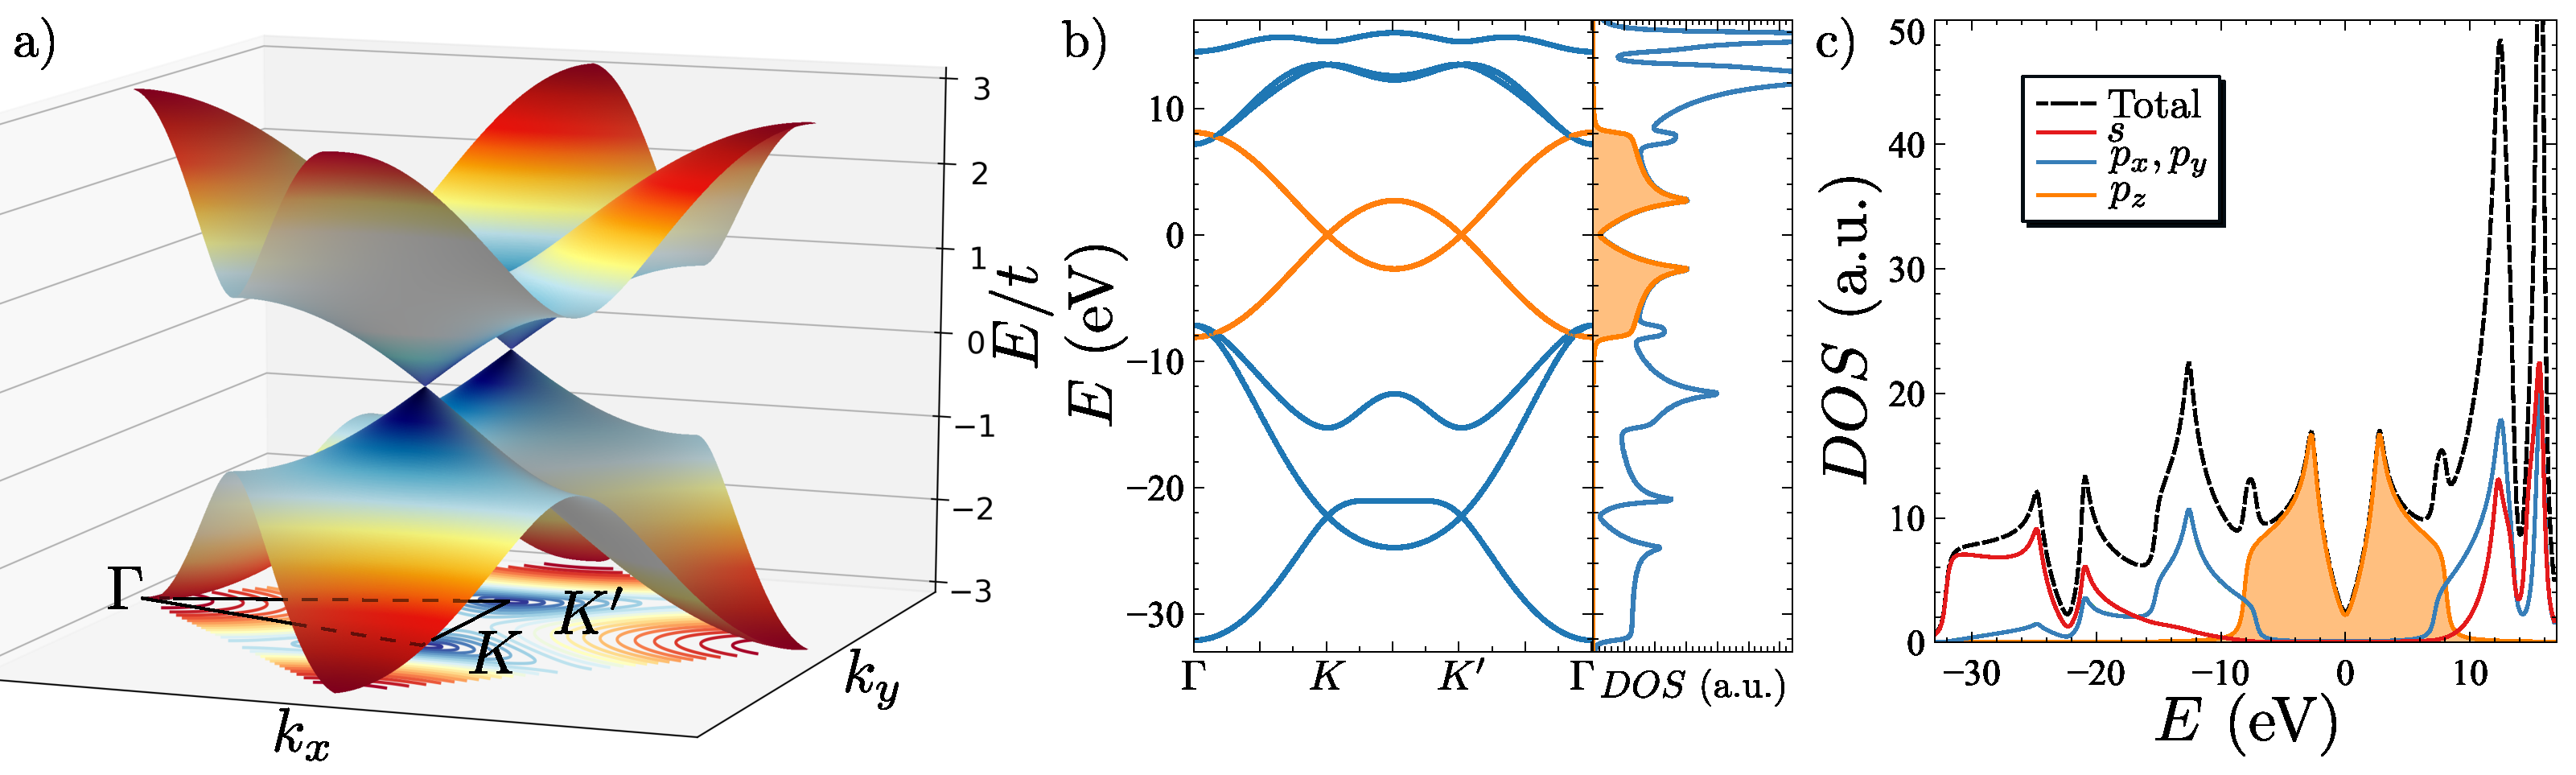
\includegraphics[width=1.1\textwidth]{graphene/figures/banddos_C.pdf}
  \makebox[\textwidth][c]{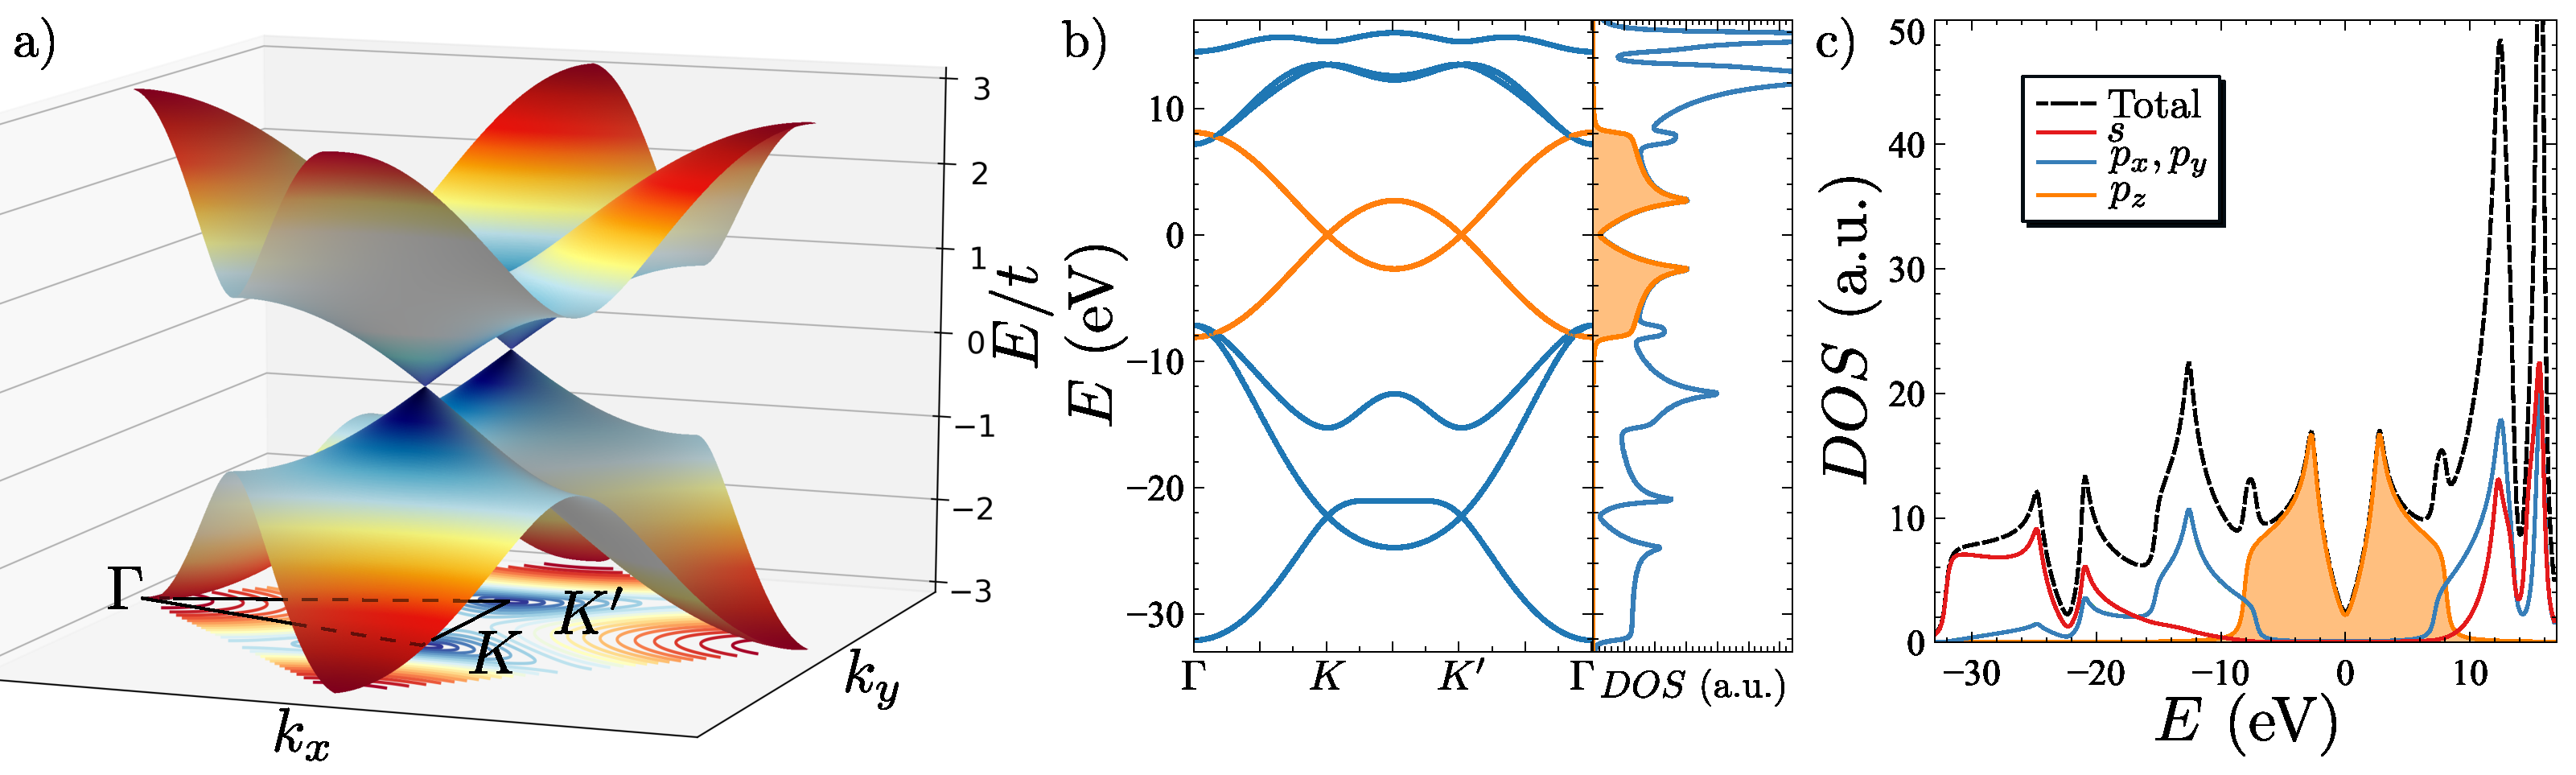
\includegraphics[width=1.2\textwidth]{graphene/figures/banddos_C.pdf}}
\end{center}
\vspace{-25pt}
\caption{a) 3D representation of the $p_z$ bands of graphene. Notice the two cones in the center of the FBZ. b) Band structure of graphene and DOS. b) DOS of graphene by orbital. Notice that the $p_x$ and $p_y$ contributions are degenerate.}
\label{bandsG}
\end{figure}
\FloatBarrier
%~~~~~~~~~~~~~~~~~~~~~~~~~~~~~~~~~~~~~~~~~~~~~~~~~~~~~~~~~~~%
In fact it is an easy exercise to calculate the band dispersion analytically. The Hamiltonian (already in the $k$-space) is:
\begin{equation}
   H(\vec{k}) = H_0 + V_1 e^{-i\vec{k}\vec{a}_1} + V_2 e^{-i\vec{k}\vec{a}_2}+
   V^{\dagger}_1 e^{i\vec{k}\vec{a}_1} + V^{\dagger}_2 e^{i\vec{k}\vec{a}_2}
\label{hk}
\end{equation}
where, in the one orbital basis $\mathcal{B}_1$ described by \eqref{basis1} can be written as
\begin{equation}
   H_0 = \left(\begin{array}{cc}
               \varepsilon_A & t \\
               t & \varepsilon_B
         \end{array}\right) \quad;\quad
   V_1 = V_2 = \left(\begin{array}{cc}
                     0 & 0 \\
                     t & 0
               \end{array}\right)
\end{equation}
which allows us to rewrite eq. \eqref{hk} as
\begin{equation}
  H(\vec{k})=\left(\begin{array}{cc}
        \varepsilon_{A} & tf(\vec{k}) \\
  tf^{\dagger}(\vec{k}) & \varepsilon_{B}
  \end{array}\right) \quad;\quad
  f(\vec{k}) = 1 + e^{-i\vec{k}\vec{a}_{1}}+
e^{-i\vec{k}\vec{a}_{2}}
\end{equation}
where we have assumed that the hopping integral between two coplanar $p_z$ orbitals is real. We have explicitly added a different on-site energy $\varepsilon_{A/B}$ for each of the sublattices

Finding the eigenvalues of $H(\vec{k})$ we obtain
\begin{equation}
  E(\vec{k})=\frac{\varepsilon_{B}-\varepsilon_{A}}{2}\pm
  \sqrt{\frac{\varepsilon^{2}_{A}+\varepsilon^{2}_{B}}{4}-
  \frac{\varepsilon_{A}\varepsilon_{B}}{2}-
  4\left(\varepsilon_{A}\varepsilon_{B}-t^2ff^{\dagger}\right) }
\end{equation}
yet in graphene these parameters vanish: $\varepsilon_{A}=\varepsilon_{B}=\varepsilon=0$ so the dispersion for the eigenvalues of the Hamiltonian:
\begin{equation}
  E(\vec{k})=\pm\sqrt{4t^2ff^{\dagger}} = \pm2|tf|
\end{equation}

%
% TODO Dirac derivation
%

\subsection{Mass}
If we were to consider not graphene but some other material with the same structure but different on-site energies for each sublattice, a so-called ``mass'' term would have to be introduced. This was hinted during the single orbital description by keeping the hypothetical on-site energies.
The main effect of such a term is to open a trivial gap at the Dirac points.

\subsection{Zeeman}
The application of an external magnetic field usually has several effects in a material. While a lot of interesting Physics is developed around the formation of Landau levels, we will restrict our study to the simpler case of the Zeeman splitting of the energy levels. This effect consists of a symmetric splitting of up ($\uaw$) and down ($\daw$) spin, resulting in a vertical shift the bands for each spin flavor.

\subsection{Spin-Orbit coupling}
\label{sec:soc}
The \acf{soc} is relativistic interaction that can be interpreted in classical terms (allowing the existence of spin in classical physics) as the interaction between the spin of the electron and the electrostatic potential of the nucleus.

In most of this section we are going to use the four orbital basis \eqref{basis4} with the geometry of \fref{graphene_summary}b), also described in the firs section of the chapter. Our Hamiltonian will have two atoms per unit cell and four orbitals per atom, so it will be a $8\times8$ matrix. When interactions concerning the spin are taken into account, the basis will be doubled with the following order:
\begin{equation}
  \mathcal{B}^{s}_4 = \left\{
  \ket{\phi^1_{s\uaw}},
  \ket{\phi^1_{s\daw}},
  \ket{\phi^1_{p_x\uaw}},
  \ket{\phi^1_{p_x\daw}},
  \ket{\phi^1_{p_y\uaw}},
  \ket{\phi^1_{p_y\daw}},
  \dots,
  \ket{\phi^n_{p_z\uaw}},
  \ket{\phi^n_{p_z\daw}}
  \right\}
\label{basis4spin}
\end{equation}

So the Hamiltonian term can be written as follows:
\begin{equation}
   H_{SO}= \lambda_{SO}\vec{L}\vec{S}
\label{soc}
\end{equation}

which is often rewritten as
\begin{equation}
   H_{SO} = \lambda_{SO}\left[L_zS_z+
   \frac{1}{2}\left(L^{+}S^{-}+L^{-}S^{+}\right)\right]
\end{equation}
just by taking into account the relations
\begin{equation*}
   S^{+} = S_x + iS_y \quad;\quad
   S^{-} = S_x - iS_y
\end{equation*}

%~~~~~~~~~~~~~~~~~~~~~~~~~~ FIGURE ~~~~~~~~~~~~~~~~~~~~~~~~~%
\begin{figure}[h!]
\centering
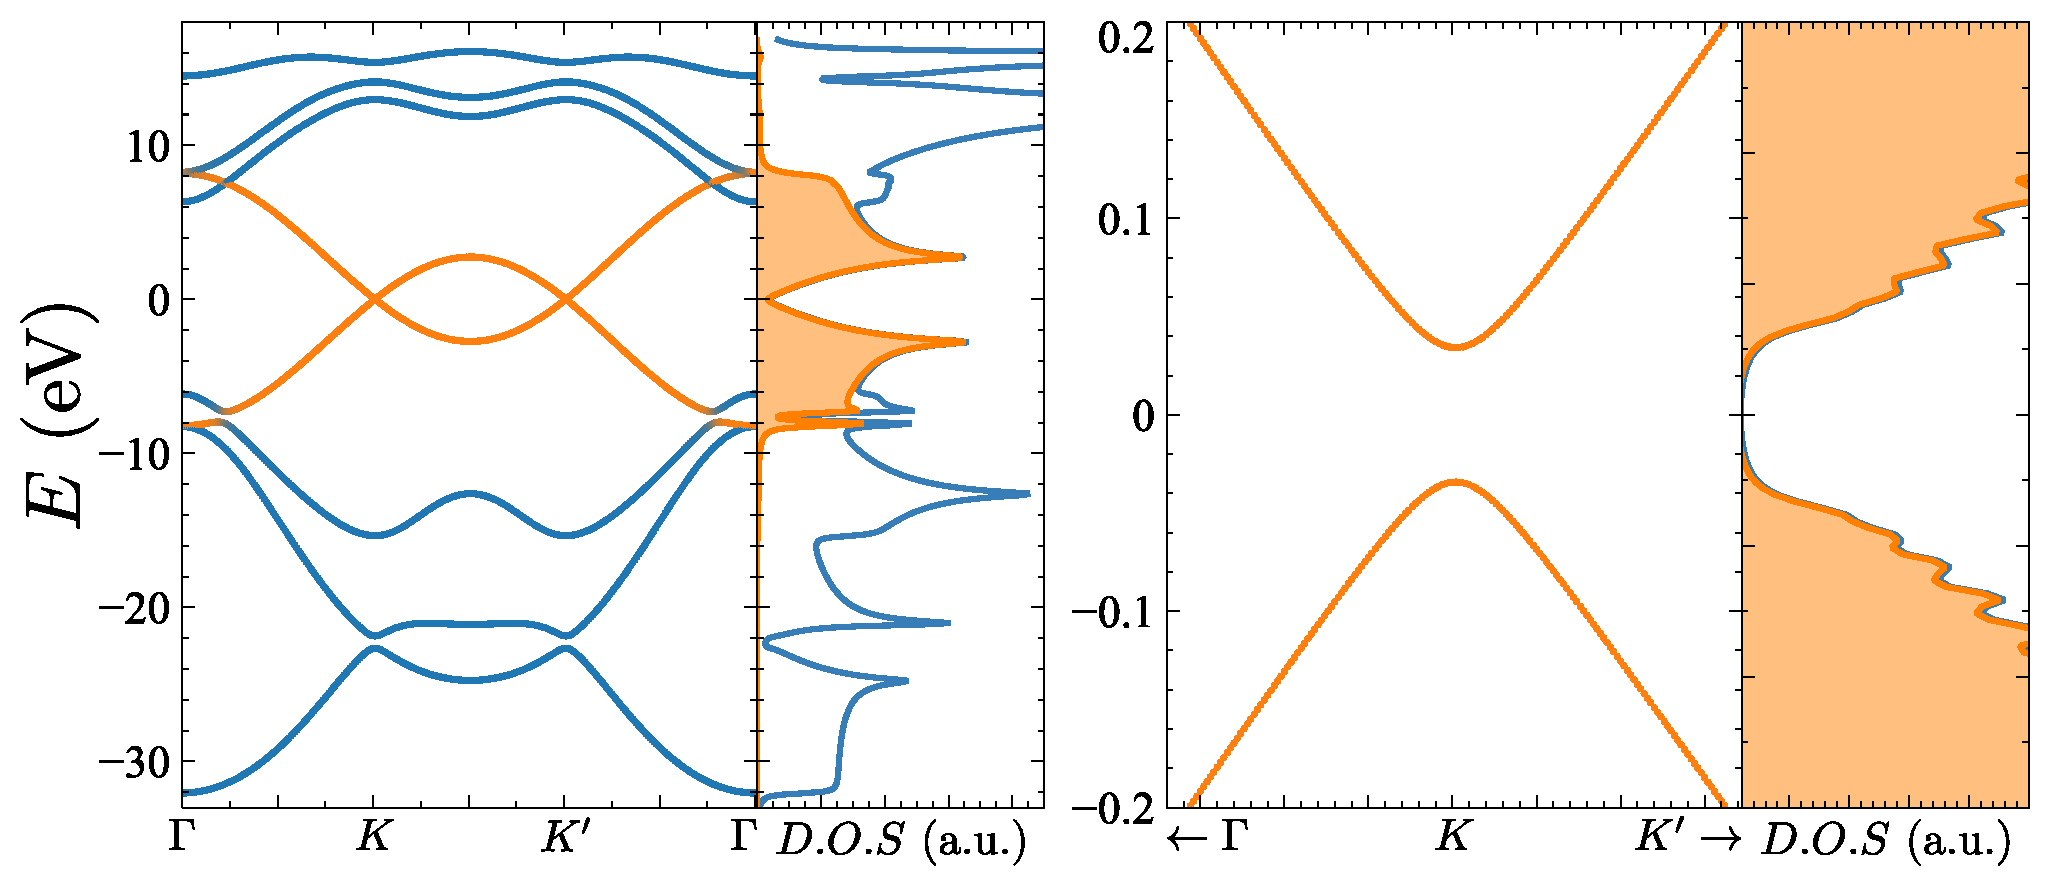
\includegraphics{graphene/figures/banddos_SOC.pdf}
\vspace{-5pt}
\caption{a) Graphene band structure in the presence of \ac{soc}. The gap due to \ac{soc} is not visible at this scale but the mixing of the $p_z$ orbital with the $\sigma$-bands becomes apparent near the $\Gamma$. The value used here is completely unrealistic with the porpoise of an easier visualization. b) Zoom to the surroundings of the Dirac point. A gap is }
\label{fig:SOC}
\end{figure}
\FloatBarrier
%~~~~~~~~~~~~~~~~~~~~~~~~~~~~~~~~~~~~~~~~~~~~~~~~~~~~~~~~~~~%

\subsection{Electric field and Rashba}
An electric field has several effects, that will be discussed later on along the thesis. It should suffice for now to discuss briefly the two main consequences.
The first feature is that an electric field would deform the atomic orbitals, breaking the mirror symmetry that protects the $\pi$-manifold. The breaking of this symmetry opens an effective channel for mixing $s$ and $p_z$ orbitals.

This effect, alongside the \ac{soc} opens a spin-flip channel via the following process: an $\uaw$ electron in a $p_z$ can transition to a $s$ orbital in the same atom, then to a $p_{x/y}$ orbital, which is connected via \ac{soc} with a $p_z$ with spin $\daw$.

We will neglect this process since both the mixing of the $s$ and the $p_z$ orbital\cite{Min2006} and the \ac{soc}\cite{Kane2005, Yao2007, Boettger2007,Gmitra2009} are quite small.

If we consider bilayer graphene, the application of an electric field has another important effect. It shifts the on-site energy of each layer which results in an opening of a gap in the band structure. This results in a very useful feature that will be exploited throughout the thesis.


\subsection{Interlayer}
The last term that we will be interested in is the interlayer coupling when the system is formed by more than one layer of graphene. This term and its effects will be discussed later on, so we will just hint here an interesting way to think about it, leaving for later a deeper analysis.

We can consider the adiabatic formation of bilayer graphene (or $n$-layer graphene, for that matter) by considering two layers of graphene infinitely apart and bringing them together.
We can use the following basis to describe such a system:
\begin{equation}
  \mathcal{B}_1 = \left\{\ket{\phi_{1A}}, \ket{\phi_{1B}},
                        \ket{\phi_{2A}}, \ket{\phi_{2B}}\right\}
\label{basis_bi}
\end{equation}
where the numbers label the layer and the letters the sublattice.

Since the two layers are infinitely apart, we can consider no interaction between them, hence we can describe the Hamiltonian of the system at the initial moment as two disconnected sectors of the same Hamiltonian, equivalent to the limit $\eta\rightarrow0$ in eq.~\eqref{Gbi}. The Hamiltonian in the one orbital basis $\mathcal{B}_1$ reads:
\begin{equation}
  H = \left(\begin{array}{cc|cc}
     0 & tf(\vec{k}) & 0 & 0 \\
     tf(\vec{k}) & 0 & 0 & 0 \\ \hline
     0 & 0 & 0 & tf(\vec{k}) \\
     0 & 0 & tf(\vec{k}) & 0
  \end{array}\right) + 
  \eta \left(\begin{array}{cc|cc}
     0 & 0  & 0  & 0 \\
     0 & 0  & t' & 0 \\ \hline
     0 & t' & 0  & 0 \\
     0 & 0  & 0  & 0
  \end{array}\right)
\label{Gbi}
\end{equation}
$\eta\in[0,1]$ will be used as a dummy parameter to switch on and off the interlayer coupling adiabatically.
When a more complex basis is used, all the \ac{sk} parameters will be scaled so that the interlayer hopping among $p_z$ orbitals is $t'=\SI{0.4}{\eV}$ in accordance with the literature\cite{KatsnelsonBook}.



%
%%%%%%%%%%%%%%%%%%%%%%%%%%%%%%%%%%%%%%%%%%%%%%%%%%%%%%%%%%%%%%%%%%%%%%%%%%%%%%%%
%%%%%%%%%%%%%%%%%%%%%%%%%%%%%%%%%%%%%%%%%%%%%%%%%%%%%%%%%%%%%%%%%%%%%%%%%%%%%%%%
\section{Quantum Spin Hall}
\subsection{Homogeneous multilayers}\label{Homogeneous}

Monolayer graphene consists of a triangular lattice with two atoms per unit cell that leads, in the reciprocal space, to a hexagonal Brillouin zone that hosts Dirac cones in its corners.
When $N$ layers are considered the crystalline structure remains the same, only there will be $2N$ atoms per unit cell. We shall only use the so called Bernal stacking, shown in  Fig.~\ref{Structure}, which is the ground state configuration, according to both \ac{dft} calculations and experimental evidence~\cite{Norimatsu2010,Charlier1994,Charlier1994a}. In Bernal stacked materials an atom from the sublattice $B$($A$) sits on top of an atom belonging to the other sublattice $A$($B$).
For $N=2$ there is only one way to achieve this, but for $N>2$ there are different possible stacking orders. In figure~\ref{Structure} we show the different possibilities for $N\leq4$, with a self-evident notation.

%~~~~~~~~~~~~~~~~~~~~~~~~~~ FIGURE ~~~~~~~~~~~~~~~~~~~~~~~~~%
\begin{figure}[h!]
\centering
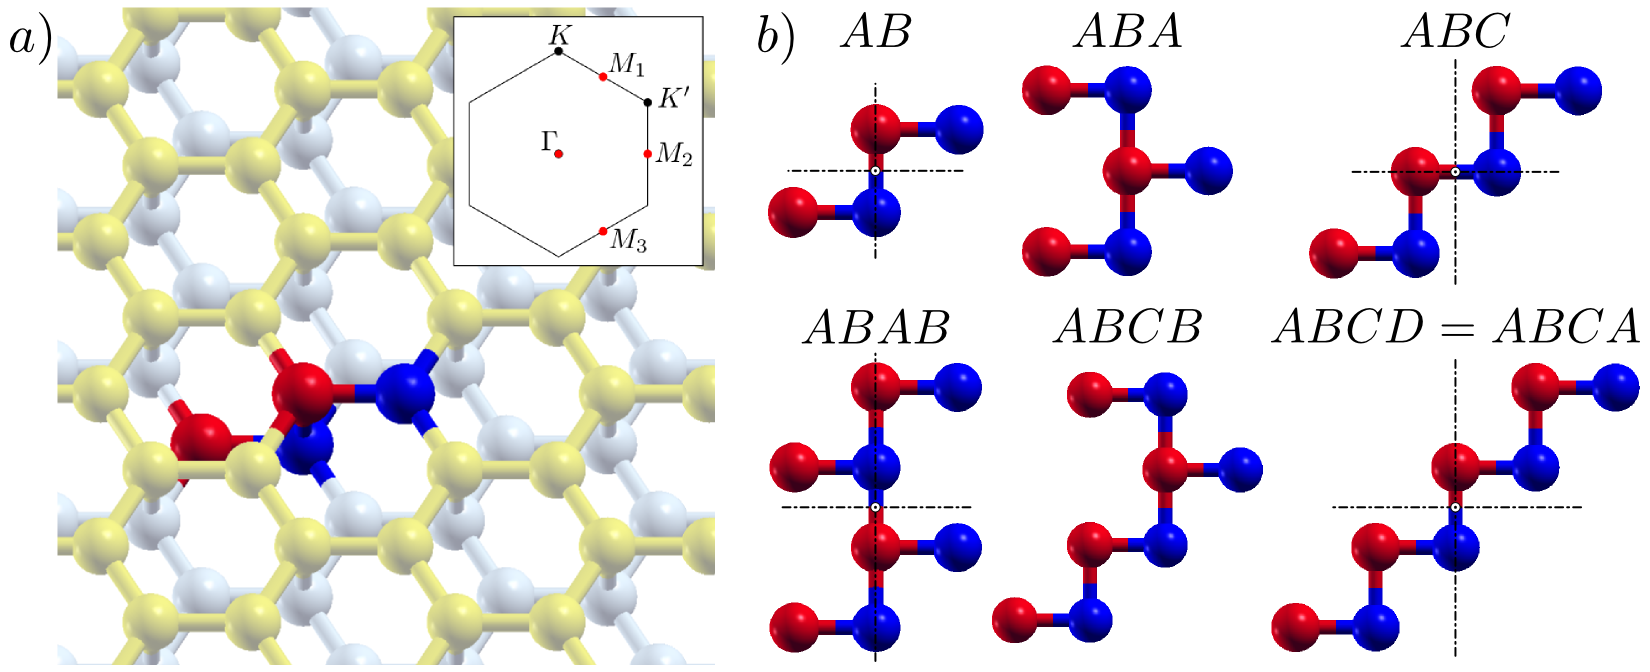
\includegraphics{chapter04/figures/structure.png}
\caption{$a)$ Crystal structure of bilayer graphene system with a highlighted unit cell. Different colors for each layer are used to distinguish the two layers. In the inset the first Brillouin Zone is depicted with the high symmetry points and the Time Reversal Invariant Momenta colored in red. In $b)$ Side view of the unit cells for all the different stackings studied. For the stackings with inversion symmetry the inversion center is shown at the crossing point of the dashed lines. For both figures red and blue denote sublattice.}
\label{Structure}
\end{figure}
%~~~~~~~~~~~~~~~~~~~~~~~~~~~~~~~~~~~~~~~~~~~~~~~~~~~~~~~~~~~%

\subsubsection{The Model}
We describe the multilayers with the following tight-binding Hamiltonian:
\begin{equation}
 H = H_{ML} + \eta H_{inter} + \lambda\vec{L}\cdot\vec{S}
\label{Hamil}
\end{equation}
where $H_{ML}$ and $H_{inter} $ account for the intralayer and interlayer  hoppings, respectively, and the last term is the intra-atomic \ac{soc}. Our tight-binding model is based on four atomic orbitals,  $s$, $p_{x}$, $p_{y}$ and $p_{z}$.
Both the intralayer and interlayer hoppings are described within the \acf{sk} formalism~\cite{Slater1954}. The intralayer hopping parameters are taken from Ref~\cite{Gosalbez-Martinez2011}. In order to study the effect of interlayer coupling, the interlayer terms are scaled by a dimensionless parameter $\eta$. When $\eta=1$, the ratio between interlayer and intralayer $V_{pp\pi}$ in graphene is taken as~\cite{Katsnelson2012} 0.13. Unless otherwise stated, in all our calculations we have $\eta=1$.
Within this model, the dimension of the Hilbert space for the minimal unit cell of the crystal with $N$ layers is $4\times2\times2\times N = 16N$ (4 orbitals per atom, 2 atoms per layer, plus the two possible spin orientations).

Without \ac{soc}, this model reproduces the very well known band structure of graphene ($N=1$) and multilayer graphene $N>1$, that portraits these systems as zero-gap semiconductors. Within this model, \ac{soc} is known to open a gap in the monolayer~\cite{Min2006}  as well as in the bilayer~\cite{Konschuh2012,Guinea2010,Cortijo2010}. In the case of the monolayer graphene the gap is known to be topological. Within this model, the computed value of the gap $\SI{1.46}{\micro\eV}$ when we take a realistic value of the atomic \ac{soc}, $\lambda=\SI{10}{\meV}$. This gap is much smaller than the ones obtained with accurate \ac{dft} calculations~\cite{Konschuh2011a}, in the range of $\sim\SI{30}{\micro\eV}$.
The reason for the discrepancy turns out to be that the mayor contribution to the \ac{soc} gap at the Dirac point comes from the coupling to the higher energy $d$ bands~\cite{Konschuh2012,Konschuh2011a}.
The later is a simple consequence of the fact that \ac{soc} opens a gap in second order in the coupling in the Dirac points when projected over the $p$ band. In comparison, \ac{soc} acts as first order when considering channels involving the $d$ band.
Nevertheless, interlayer hopping may open a first order spin flipping channel in the $p$ manifold, becoming of the same order as the intrinsic spin conserving $d$-level contribution.
These last processes would be the ones missing in the multilayer Kane-Mele model, and should be added for completeness.
In our case, for the sake of simplicity, we will focus on the spin flipping channel, and use a four orbital tight-binding model considering $\lambda$ as a free parameter.

Future work shall focus on the effect of the d-levels in multilayer graphene, which will not be addressed here.

\begin{figure*}
\begin{minipage}{.9\linewidth}
\begin{center}
 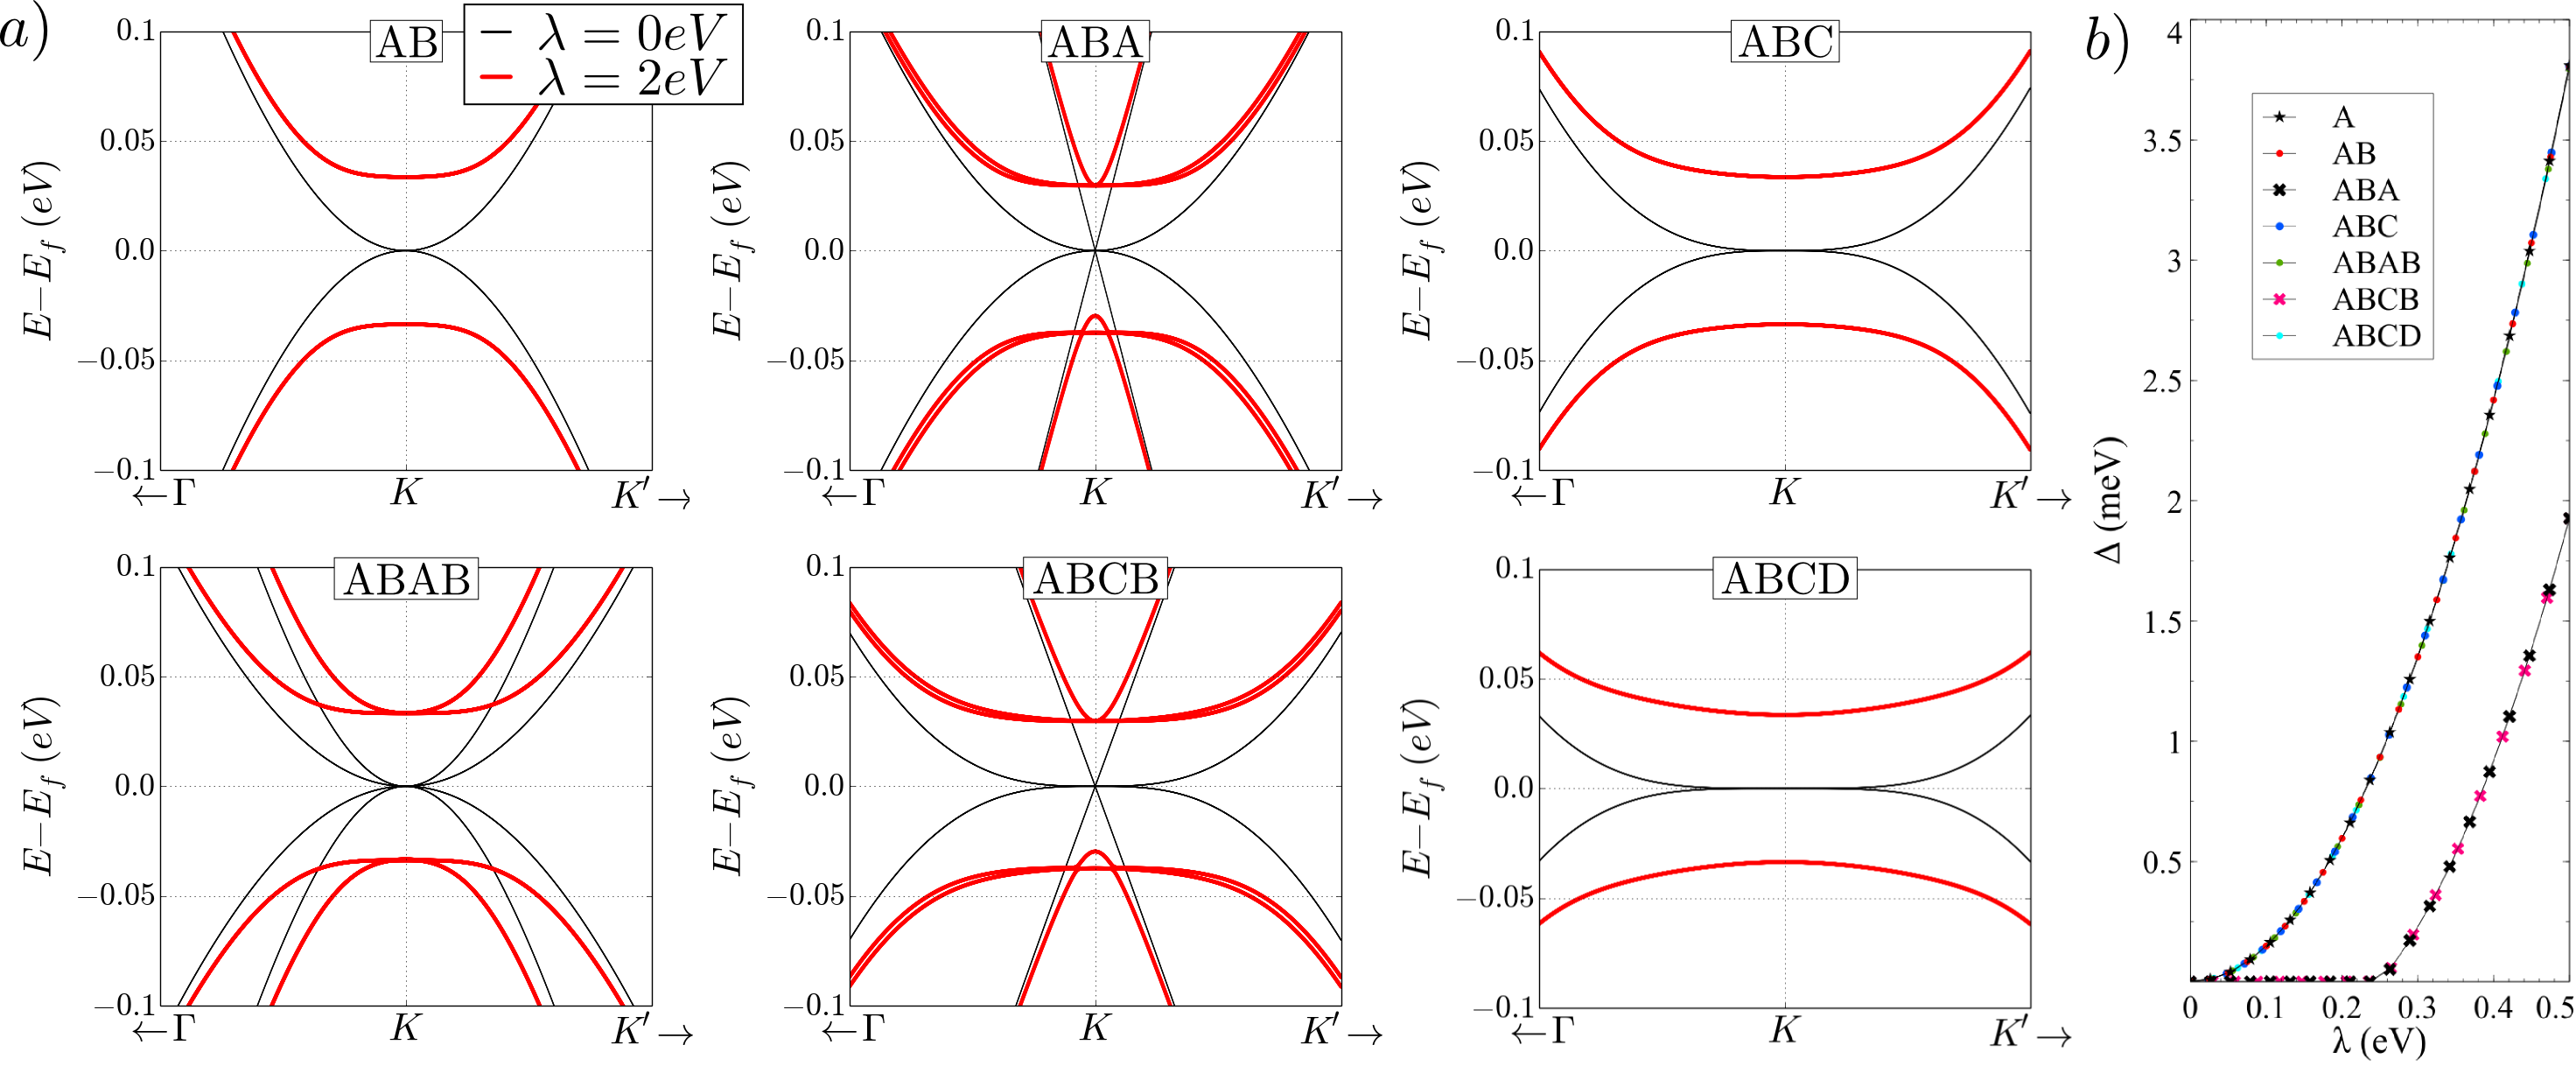
\includegraphics[width=\textwidth]{chapter04/figures/bands.png}
\end{center}
\end{minipage}
\caption{ In $a)$ the band structure close to the $K$ point is shown for all the possible stackings of multilayer graphene with $N = {2,3,4}$. Only when $\lambda \neq 0$ (red line) a gap is opened at the Dirac points.
Note that for $ABA$ and $ABCB$ stackings there are linear bands when $\lambda=0$ that when the \ac{soc} is switched on cause a smaller gap than in the other cases.
In $b)$ the dependence of the gap with the \ac{soc} $\lambda$ is shown. The anomalous behavior for the $ABA$ and $ABCB$ stackings is just due to the linear bands mentioned before.}
\label{Bilayer}
\end{figure*}

The effect of \ac{soc} on the band structure of the multilayers can be summarized in the following points:
\begin{enumerate}
\item \ac{soc}  opens up a gap for all the $N$ stacked layers considered, reproducing the existing results~\cite{Guinea2010} for the case of $N=2$.
Notice that in the case of $ABA$ and $ABCB$ stackings, the system remains gapless until a critical value of $\lambda$.
This peculiarity is related to the non uniform evolution of the SO splitting of the linear and non-linear bands  as shown in figure~\ref{Bilayer}.


\item  The scaling of the gap with $\lambda$ is very similar for monolayer and $N=2,3,4$ multilayers as it is shown in Figure~\ref{Bilayer}. Therefore, it is expected that within this model, the gap opened by the intrinsic \ac{soc} might be as small in multilayers as in monolayers.

\item The magnitude of the band-gap is insensitive to the interlayer coupling. This result is somewhat surprising, since together with atomic \ac{soc} the interlayer coupling opens a spin-flip channel, otherwise missing in the monolayer case.
For the $AB$ bilayer, this can be understood considering the Hamiltonian at the Dirac point, for a given spin flavor. In the basis $\{A_{1},B_{1},A_{2},B_{2}\}$
the low energy Hamiltonian is given by
\begin{equation}
H(K) = \left(\begin{array}{cccc}
\Delta/2 &     0   &    0   &     0 \\
   0   & -\Delta/2 &  \eta t  &     0 \\
   0   &\eta t^{\dagger}&\Delta/2&  0 \\
   0   &     0   &    0   & -\Delta/2
   \end{array}\right)
\end{equation}
where $\Delta$ is the SO gap. When $\eta=0$ this Hamiltonian represents two decoupled monolayers.
For finite $\eta$ the eigenvalues are $E^{1}_{\pm}=\pm\Delta/2$ and $E^{2}_{\pm}=\pm\sqrt{(\eta t)^{2}+(\Delta/2)^{2}}$.
Since $\eta t\gg\Delta$ the gap is still controlled by the $E^{1}$ couple and thereby identical to that of the decoupled monolayers.
As a result, switching on the interlayer coupling does not close the \ac{soc} gap of the monolayer as shown in Figure~\ref{Bilayer}. As a consequence,  the ground state of two decoupled ($\eta=0$) monolayers can be adiabatically connected to the ground state of the bilayer ($\eta=1$).
\end{enumerate}

The last observation leads to the following result: odd $N$ stacked graphene will be quantum spin Hall Insulators, whereas  even $N$ will not. More precisely, for a system of $N$ decoupled monolayers the $Z_{2}$ invariant is:
\begin{equation}
 Z_{2}(N) = \left[Z_{2}(1)\right]^{N}
 \label{trivial}
\end{equation}
Since the gap opened by $\lambda$ remains unaffected when switching on the interlayer coupling $\eta$, the value of $Z_2$ for graphene-like multilayers is also given by equation~\eqref{trivial}.
We have verified that this qualitative behavior remains unchanged when $d$-channels are included in the picture by performing all-electron \ac{dft} calculations. %\cite{elk}.  %XXX CITE ELK
In the realistic low $\lambda$ limit, the gap is controlled by the linear contribution in $\lambda$, namely the $d$-channel. For large SO, the quadratic in $\lambda$ $p$-channel becomes dominant, which corresponds to the situation in which the gap opening is properly captured by the \ac{sk} model.
Thus, by artificially increasing $\lambda$ in a \ac{dft} calculation, it is possible to move from the $d$-dominated to the $p$-dominated SO gap. We have obtained that both limits are adiabatically connected without gap closing, so that the topological properties in the low $\lambda$ limit are the same than in the large $\lambda$ limit.

In the following we verify equation~\eqref{trivial} using two different strategies. In the case of inversion symmetric structures, we compute the $Z_2$ invariant. In all cases, we compute the edge states and check whether they fill the gap, or else.  Independently on how the topological character is obtained, eq.~\eqref{trivial} holds in all the cases.



\subsection{Calculation of the $Z_{2}$ invariant.}
Using the method developed by Fu and Kane in 2007~\cite{Fu2007} for systems with
inversion symmetry it is possible to determine easily its topological character
(the $Z_{2}$ invariant) by calculating the parity of the occupied Bloch wave
functions at the time reversal invariant momenta (TRIMs).

\begin{equation}
\delta_{i} = \displaystyle\prod^{N}_{m=1}\xi_{2m}(\Gamma_{i}) \quad;\quad (-1)^{\nu} = \prod_{i}\delta_{i}
\end{equation}
where $\xi_{2m}$ is the parity eigenvalue of the $2m^{th}$ occupied state at the TRIM $\Gamma_{i}=\{\Gamma,M_{1},M_{2},M_{3}\}$. Using this method the topological character of a system will be determined just by the quantity $(-1)^{\nu}$, resulting that $(-1)^{\nu}=+1$ means trivial topology and $(-1)^{\nu}=-1$ means non trivial topology.
The calculation for the systems with inversion symmetry yields the following results:
\begin{center}
 \begin{tabular}{ c | c c c c c}
              &  A  &  AB & ABC & ABAB & ABCD \\\hline
     $M_{1}$  & $+$ & $+$ & $+$ &  $+$ &  $+$  \\
     $M_{2}$  & $+$ & $+$ & $+$ &  $+$ &  $+$  \\
     $M_{3}$  & $+$ & $+$ & $+$ &  $+$ &  $+$  \\
     $\Gamma$ & $-$ & $+$ & $-$ &  $+$ &  $+$  \\\hline
 $(-1)^{\nu}$ & $-$ & $+$ & $-$ &  $+$ &  $+$
 \end{tabular}
\label{parity}
\end{center}

This guarantees that $A$ and $ABC$  crystals are topological but the bilayers and tetralayers (with inversion symmetry) are not.
%This method cannot be applied to systems without inversion symmetry,  which are addressed in the next section using a different approach.
For systems without inversion symmetry, the calculation of the $Z_{2}$ invariant requires a different approach~\cite{Fu2006, Fukui2005, Fukui2007} that requires a line integral of the Berry curvature over a contour in the Brillouin zone. Instead, we compute the edge states for these systems and invoke the bulk-edge correspondence to address the topological nature of those systems.


\subsection{Edge states}
To confirm equation \eqref{trivial} even for systems without inversion symmetry we look for the presence of gapless edge states.
We consider armchair-terminated  semi-infinite crystals.  Using translation invariance along the direction parallel to the edge, we block-diagonalize  the Hamiltonian of the semi-infinite 2D  crystal in terms of a collection of $k_{||}$ dependent semi-infinite 1D Hamiltonians, as indicated in figure~\ref{Mapping}. The 1D Hamiltonian describes unit cells with $4N$ atoms, where $N$ stands for the number of graphene layers.  The intra-cell terms are denoted by $H_0(k_{||})$ and the inter-cell hoppings by $V(k_{||})$.



\begin{figure}[hbt]
 \centering
  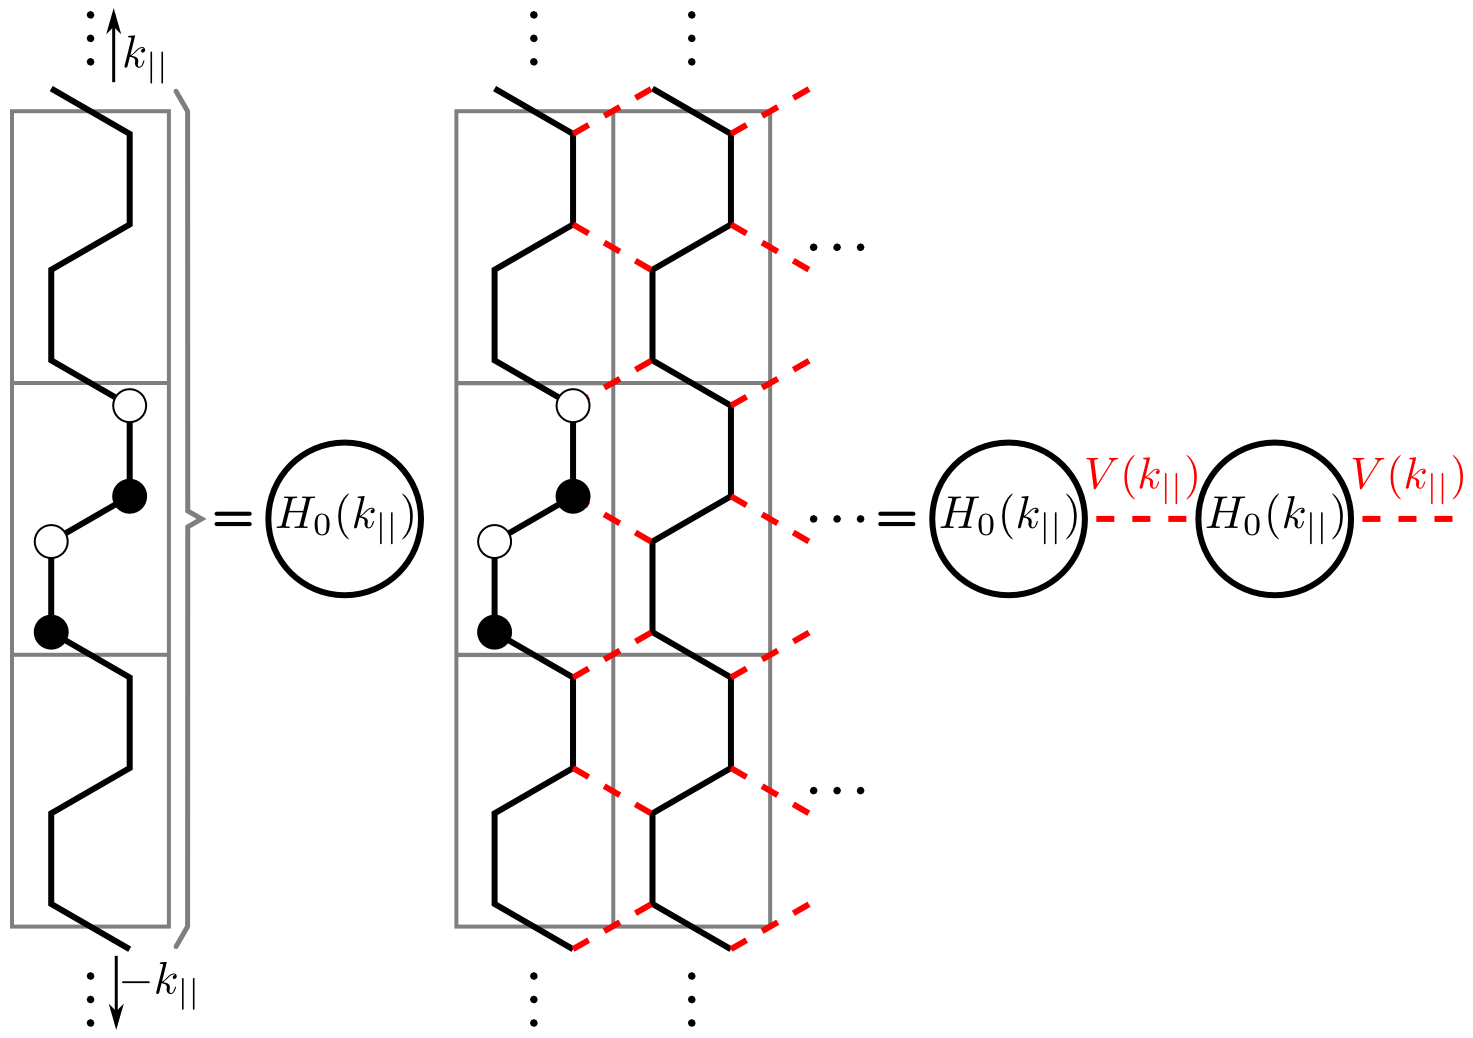
\includegraphics{chapter04/figures/seminfinite.png}
\vspace{-5pt}
\caption{Scheme of the mapping between a semi-infinite crystal and a semi-infinite chain. The coupling between each linear chain (with $k_{||}$ well defined) is introduced by means of a self energy $\Sigma_{R}$.}
\label{Mapping}
\end{figure}

\begin{figure*}
\centering
% \begin{minipage}{.85\linewidth}
% \begin{center}
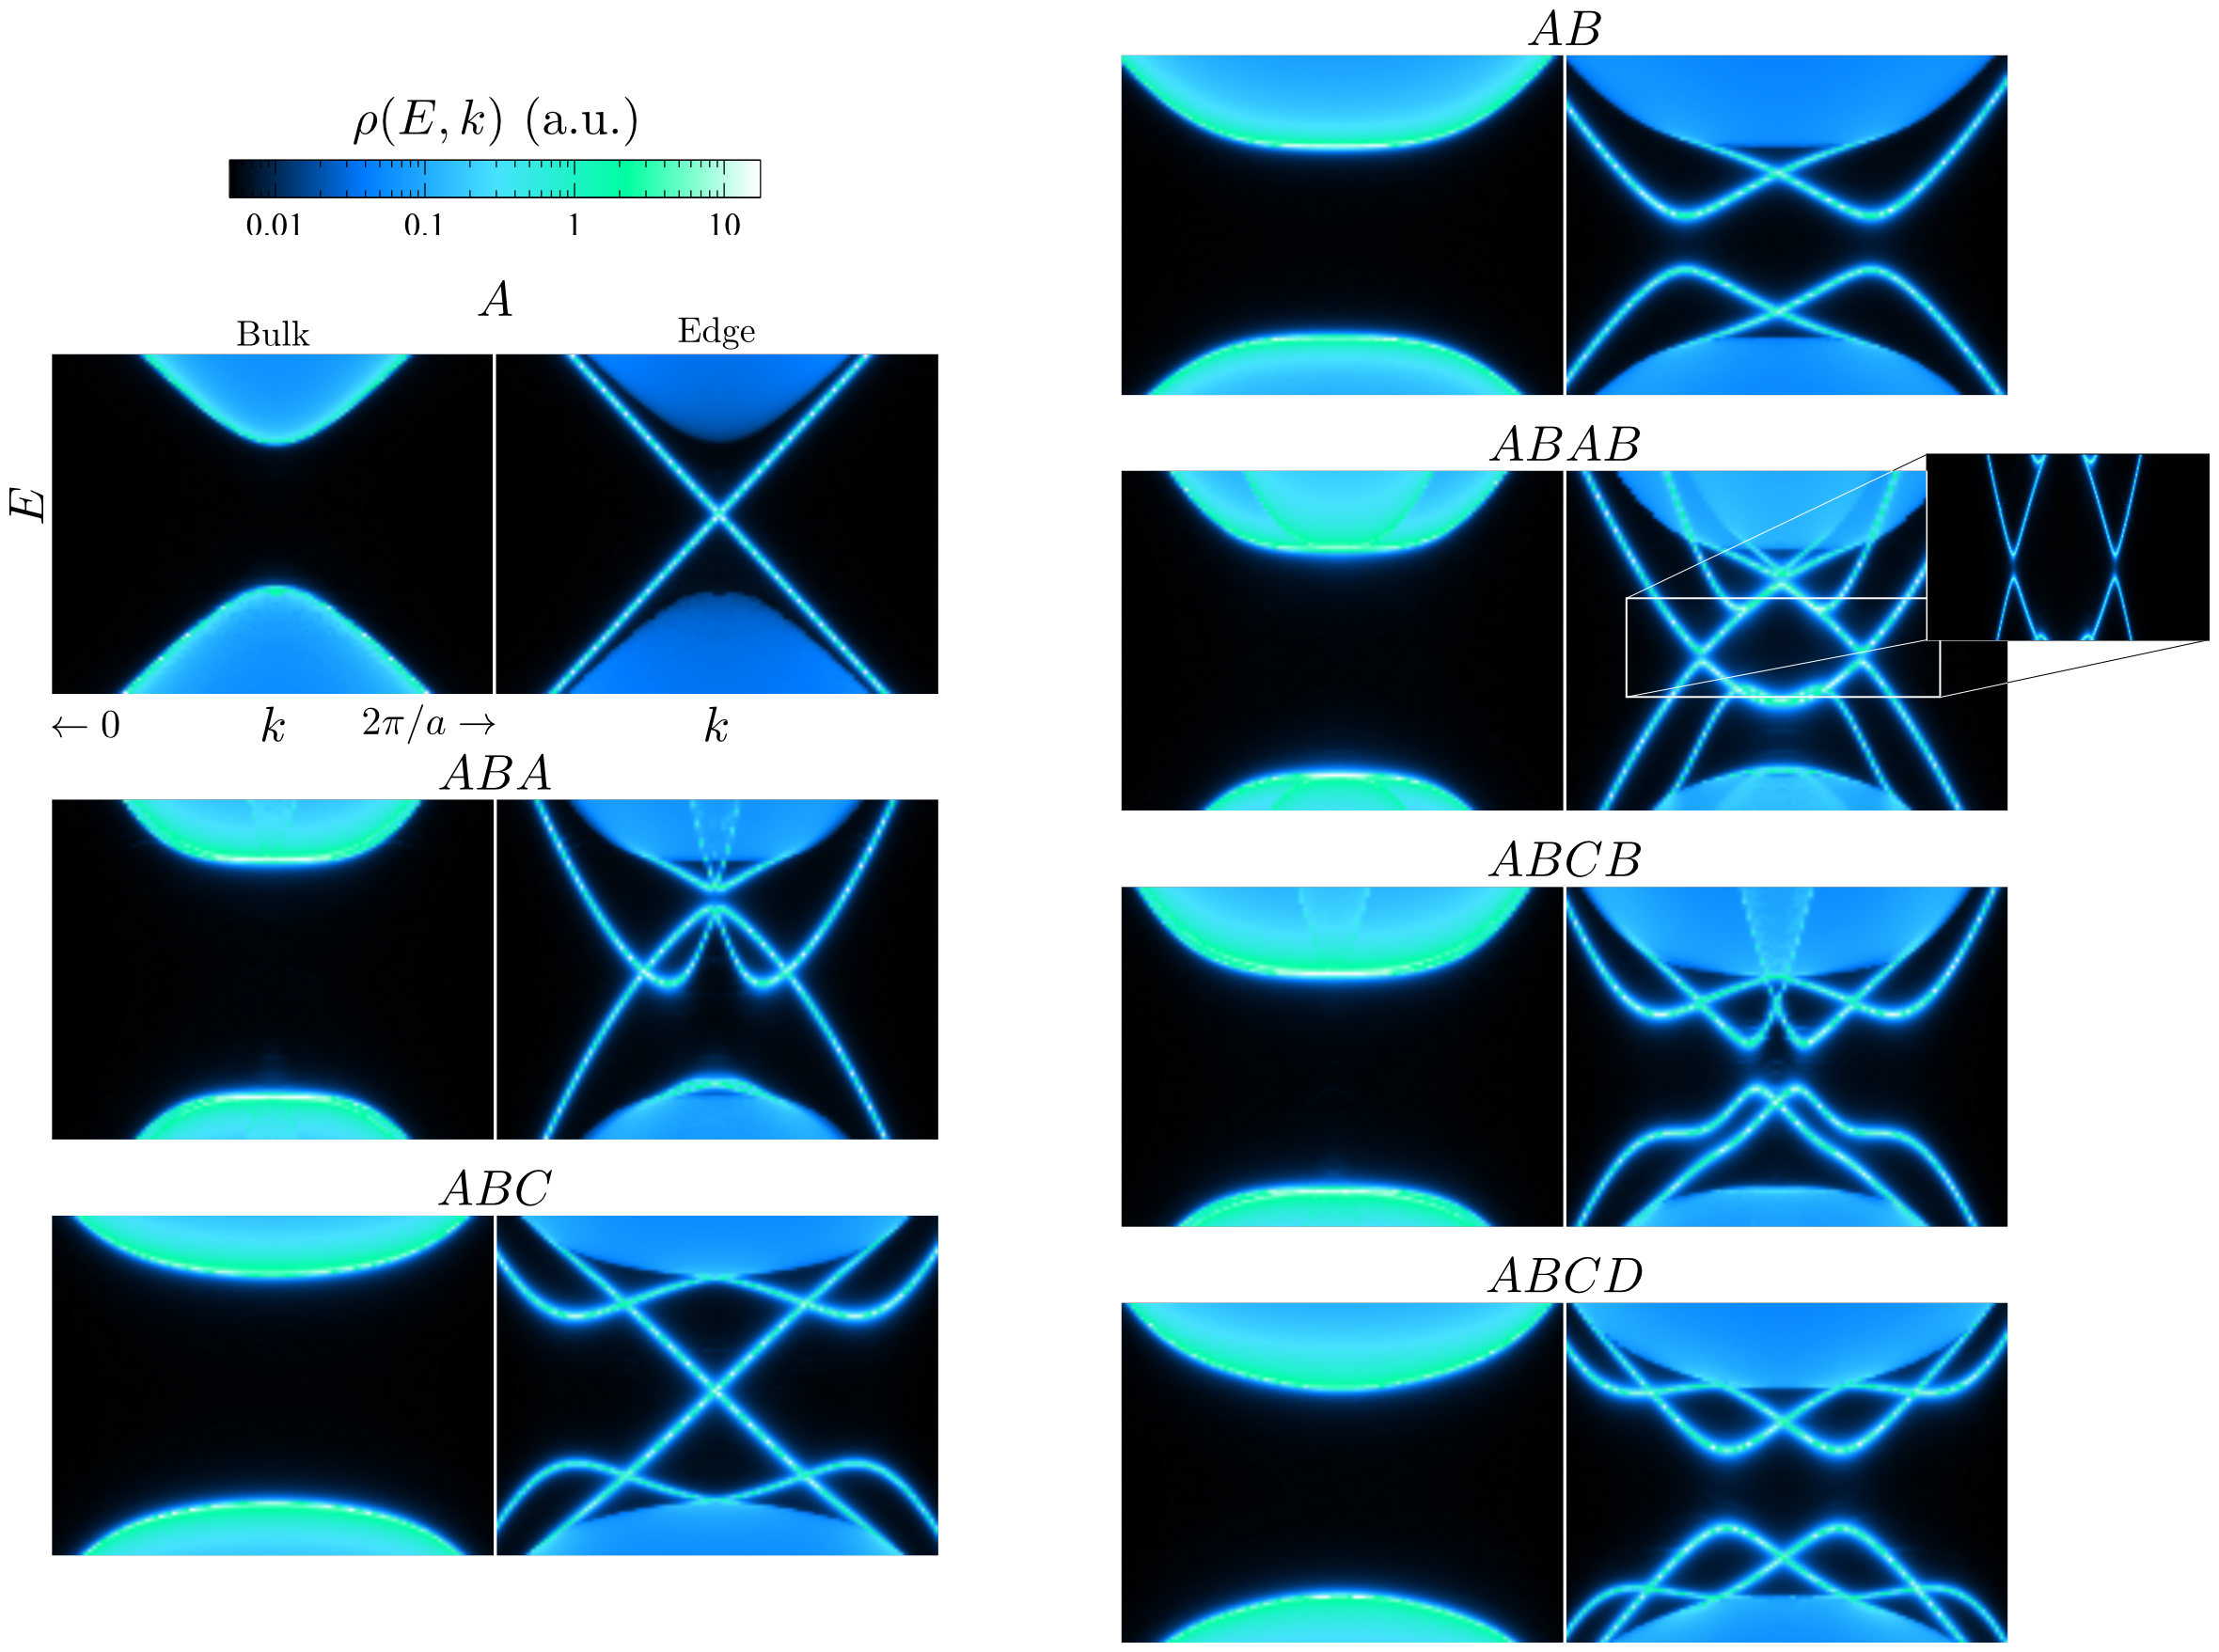
\includegraphics[width=\textwidth]{chapter04/figures/dyson.png}
% \end{center}
% \end{minipage}
\caption{For each structure bulk and edge \ac{dos} (left and right panel respectively).
Gapless edge states appear only when an odd number of layers is considered independently of the stacking used.}
\label{DOSdyson}
\end{figure*}


The surface Green function of this  block tridiagonal semi-infinite matrix can be  written as:
\begin{equation}
G^{edge}(E,k_{||}) =
\left[E+i\epsilon-H_0(k_{||})-\Sigma_{R}(k_{||})-\Sigma_{H}(k_{||})\right]^{-1}
\end{equation}
where $\Sigma_{R}(k_{||})$ is a self-energy that accounts for the coupling to the semi-infinite crystal,
$\Sigma_{H}(k_{||})$ is the self-energy due to its interaction with the $H$ atoms included to get rid of the dangling bonds and $\epsilon$ a small analytic continuation.

The self-energy $\Sigma_{R}$ can be calculated employing a recursive Green's function method that leads to the following coupled equations
\begin{eqnarray}
\nonumber \Sigma_{R}(E,k_{||})&=& V_{R}(k_{||})g_{R}(E,k_{||})V^{\dagger}_{R}(k_{||})
\\
g_{R}(E,k_{||}) &=& \left[E-H_0(k_{||}) -\Sigma_{R}(E,k_{||})\right]^{-1}
\end{eqnarray}

The $\Sigma_{H}(k_{||})$ is calculated just as an additional iteration to the self-consistent calculation with the appropriate value for the hoppings $C-H$.

For a given $k_{||}$ we compute the \ac{dos} using
\begin{equation}
 \rho(E,k_{||}) = -\frac{1}{\pi} Im[G^{edge}(E,k_{||})]
\end{equation}
Using a similar  approach we can also obtain the bulk \ac{dos}  calculating the bulk Green function by recursion.

In figure~\ref{DOSdyson} we show the \ac{dos} for both bulk and edge for all the stackings as a contour plot in the $k_{||},E$ plane. For each stacking the left panel shows the bulk \ac{dos}, which are gaped for all the stackings and the right panel shows the edge states.  The calculations are done for a rather large value of $\lambda=\SI{2}{\eV}$. The first thing to  notice is that, for such large values of $\lambda$, all the structures have edge states. However, only in the case of odd $N$, shown in the left column, the in-gap states are gapless.  This is a necessary condition in order to have a \ac{qshi}.  In contrast,  all systems with even $N$ have edge states with a gap. Thereby, they are definitely not in the \ac{qsh} phase, validating
 equation~\eqref{trivial}. Therefore, we conclude that odd  $N$ graphene stacks are \ac{qshi} and even $N$ are trivial insulators. In all cases, the gap opened by \ac{soc} is quite small.



%%%%%%%%%%%%%%%%%%%%%%%%%%%%%%%%%%%%%%%%%%%%%%%%%%%%%%%%%%%%%%%%%%%%%%%%%%%%%%%%
\subsection{Heterogeneous multilayers}
\label{Heterogeneous}
In the previous section we have seen that for homogeneous multilayers the gap opened by \ac{soc} has the same magnitude than for the monolayer. Thereby, homogeneous multilayers of graphene  would not improve the prospects for observation of the \ac{qsh} phase compared to the monolayer. We thus explore the case of a heterogeneous multilayer. This is motivated in part by recent experiments~\cite{Avsar2014} that seem to indicate an enhancement of the \ac{soc} interaction in graphene due to proximity to WS$_2$, a trivial semiconductor with quite large \ac{soc} and no inversion symmetry. There has also been plenty of work studying the enhancement of \ac{soc} interaction in graphene due to proximity to heavy metals~\cite{Zhang2014a}. However, it would be much more interesting if graphene could be driven into a \ac{qsh} phase by proximity to an insulator, so that the only conducting channels would be only at the edges of graphene.

Density functional calculations show~\cite{Kaloni2014} that a topological band-gap opens in graphene on top of both $WS_2$ and $WSe_2$, two widely studied two dimensional \acp{tmd}.  The magnitude of this gap is in the range of a few meV, i.e.,  two or  three orders of magnitude larger than  the intrinsic \ac{soc} gap.

%~~~~~~~~~~~~~~~~~~~~~~~~~~ FIGURE ~~~~~~~~~~~~~~~~~~~~~~~~~%
\begin{figure}[hbt]
 \centering
  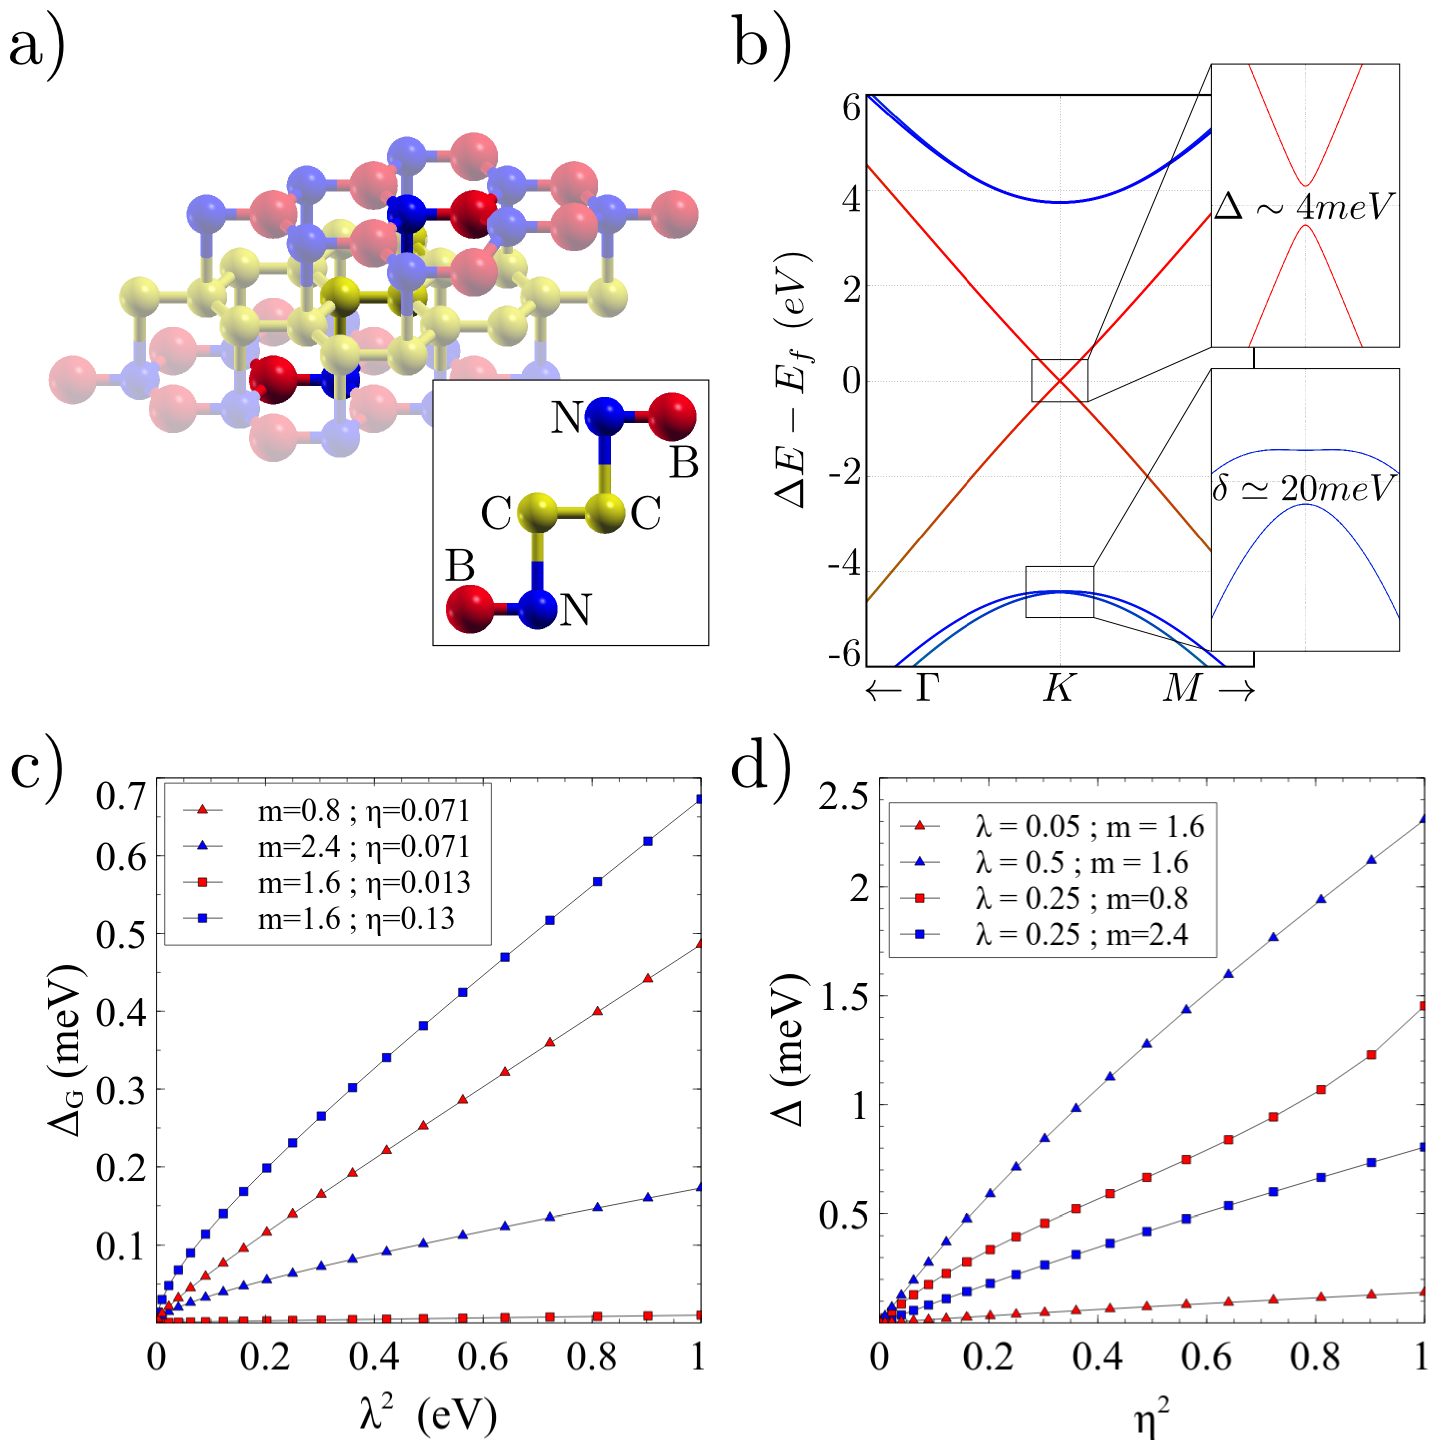
\includegraphics{chapter04/figures/encapsulated.png}
\caption{Panel $a)$ shows the structure of the heterostructure considered.
Panels (b,c,d) show the dependence of the induced gap in graphene due to the proximity of the encapsulating layers. In panel $b)$ it can be seen that the gap is proportional to $\lambda^{2}$ and this estimation gets better as the gap of insulating layers gets bigger. Panel $b)$ shows how the interlayer coupling $\eta$ produces the expected effect, for small interlayer coupling the induced gap is small but it grows quickly as $\eta$ increases. Panel $c)$ shows the dependence of the induced gap with the sublattice imbalance}
\label{induced}
\end{figure}
%~~~~~~~~~~~~~~~~~~~~~~~~~~~~~~~~~~~~~~~~~~~~~~~~~~~~~~~~~~~%

Here we propose a toy model to understand the opening of a non-trivial gap due to proximity to a trivial insulator with strong \ac{soc}.
For that matter, we take graphene encapsulated between two monolayers of a trivial semiconductor with strong \ac{soc} and broken inversion symmetry.   Specifically, the structure of  these adjacent monolayers is that of a $BN$-like crystal (see figure~\ref{induced}(a)).   The choice of the stacking is such that, globally, the structure has inversion symmetry. Otherwise,  a trivial band gap would be opened by proximity~\cite{Giovannetti2007}.

The $BN$-like crystal is described with the same interatomic \ac{sk} parameters than graphene, but very different on-site parameters. In particular we assume a large \ac{soc} $\lambda$ and a staggered potential $\pm m$ that breaks inversion symmetry of the top and bottom layers.
Since we are interested in the proximity effect, we turn off the atomic \ac{soc} of the graphene layer.
As in the case of the homogeneous multilayers, the interlayer coupling is characterized by the dimensionless parameter $\eta$.   In this case we impose
zero \ac{soc} for the graphene layer, in order to study the proximity effect.   For $\eta=0$ the bands of this system would be the superposition of those of the top and bottom insulators, with gap $2m$, and the bands of graphene, whose Dirac cones would lie inside the gap.  Broadly speaking, this picture remains the same as the interlayer coupling is turned on.    Interestingly, a non-trivial gap $\Delta$  opens in the Dirac cones only when $\eta\neq 0$ and $\lambda\neq 0$.  We have verified that this gap satisfies the  scaling
\begin{equation}
\Delta \propto \frac{\lambda \eta^2}{m^{2}}
\label{wcoupling}
\end{equation}
in the limit of small $\lambda$, $\eta$ and $m^{-1}$. This results implies that graphene can borrow \ac{soc} from a neighbor trivial insulator layer via interlayer coupling. Using the method of the TRIM  we have verified that this insulator has $Z_2=(-1)^{\nu}=-1$, and is therefore topologically non-trivial.

The magnitude of the proximity effect away from the weak coupling limit of eq. \eqref{wcoupling} is shown in figures \ref{induced}.  We study the dependence of the proximity gap $\Delta$ as a function of both the \ac{soc} $\lambda$ and the interlayer coupling $\eta$ for two values of the encapsulating layer  staggered potential $m$. It is apparent that, taking $m=\SI{2.0}{\eV}$ (a trivial gap $\sim\SI{1.5}{\eV}$) and $\lambda \simeq \SI{0.25}{\eV}$, values in line with those of 2D \ac{tmd}, the proximity gap is in the order of
 $\sim\SI{1}{\meV}$, similar to the \ac{dft} results. Therefore, our model provides a reasonable justification of the \ac{dft} computations, which are certainly more complete.

Our  toy model does not capture some probably important features of real heterogeneous multilayers.  For instance,
the interlayer interaction  could break inversion symmetry which is expected to open a trivial gap.  In addition,
the geometry of our encapsulating  layers was  chosen to minimize the size of the unit cell, rather than to describe a real material.  In general, the coupling of graphene to other 2D crystals will imply a new length scale, given by the size of the new unit cell. In this setup, the inversion symmetry breaking could average out.


% \section{Graphene bilayer}
%%%%%%%%%%%%%%%%%%%%%%%%%%%%%%%%%%%%%%%%%%%%%%%%%%%%%%%%%%%%%%%%%%%%%%%%%%%%%%%%
% \section{Conclusions}\label{conclus}
% We have studied the quantum spin Hall phase in multilayer graphene and in graphene encapsulated by a trivial semiconductor. In the case of multilayer graphene we find that only the stacks with an odd number of layers are quantum spin Hall insulators. However, the size of the gap is the same than for a monolayer, and thereby, most likely too small to be detected experimentally.
% In contrast, we propose a toy model for  graphene encapsulated between two semiconducting layers with strong SOC and a trivial gap. Our model shows that  a non-trivial gap can be opened in graphene whose magnitude is controlled by the atomic spin orbit coupling of the adjacent layers. Our model provides a qualitative understanding of recent \ac{dft} calculations~\cite{Zhang2014a} as well as recent experimental work~\cite{Avsar2014} and shows a promising route to observe the quantum spin Hall phase in graphene.
%%%%%%%%%%%%%%%%%%%%%%%%%%%%%%%%%%%%%%%%%%%%%%%%%%%%%%%%%%%%%%%%%%%%%%%%%%%%%%%%
%%%%%%%%%%%%%%%%%%%%%%%%%%%%%%%%%%%%%%%%%%%%%%%%%%%%%%%%%%%%%%%%%%%%%%%%%%%%%%%%




%%%%%%%%%%%%%%%%%%%%%%%%%%%%%%%%%%%%%%%%%%%%%%%%%%%%%%%%%%%%%%%%%%%%%%%%%%%%%%%%
%%%%%%%%%%%%%%%%%%%%%%%%%%%%%%%%%%%%%%%%%%%%%%%%%%%%%%%%%%%%%%%%%%%%%%%%%%%%%%%%
%%%%%%%%%%%%%%%%%%%%%%%%%%%%%%%%%%%%%%%%%%%%%%%%%%%%%%%%%%%%%%%%%%%%%%%%%%%%%%%%
%\section{Islands}
%With these parameters we consider an armchair hexagonal nanoisland ($\sim10^4-10^5$ $C$ atoms). Such a system is 0-dimensional, hence, no band structure can be defined but rather just the spectrum. Nevertheless, in the limit of an infinite island, the physical properties of graphene should be recovered.
%We can get an idea of how far from real graphene we are by considering the confinement gap. Graphene is famously known for not having a gap in the band structure. Graphene nanoislands do have a gap due to its finite size, but the larger the island, the smaller the gap until in the limit of an infinite island (graphene) the gap shall disappear. The dependence of the gap and the size of the island can be estimated as a free particle in a box of size $L$, roughly $\Delta\sim\frac{1}{L^2}$. Performing the actual calculation we can obtain see the dependence of the gap with the size of the island (see Fig.~\ref{confinement}) and estimate the necessary dimensions for our calculations.
%
%%~~~~~~~~~~~~~~~~~~~~~~~~~~ FIGURE ~~~~~~~~~~~~~~~~~~~~~~~~~%
%\begin{figure}[h!]
%  \centering
%  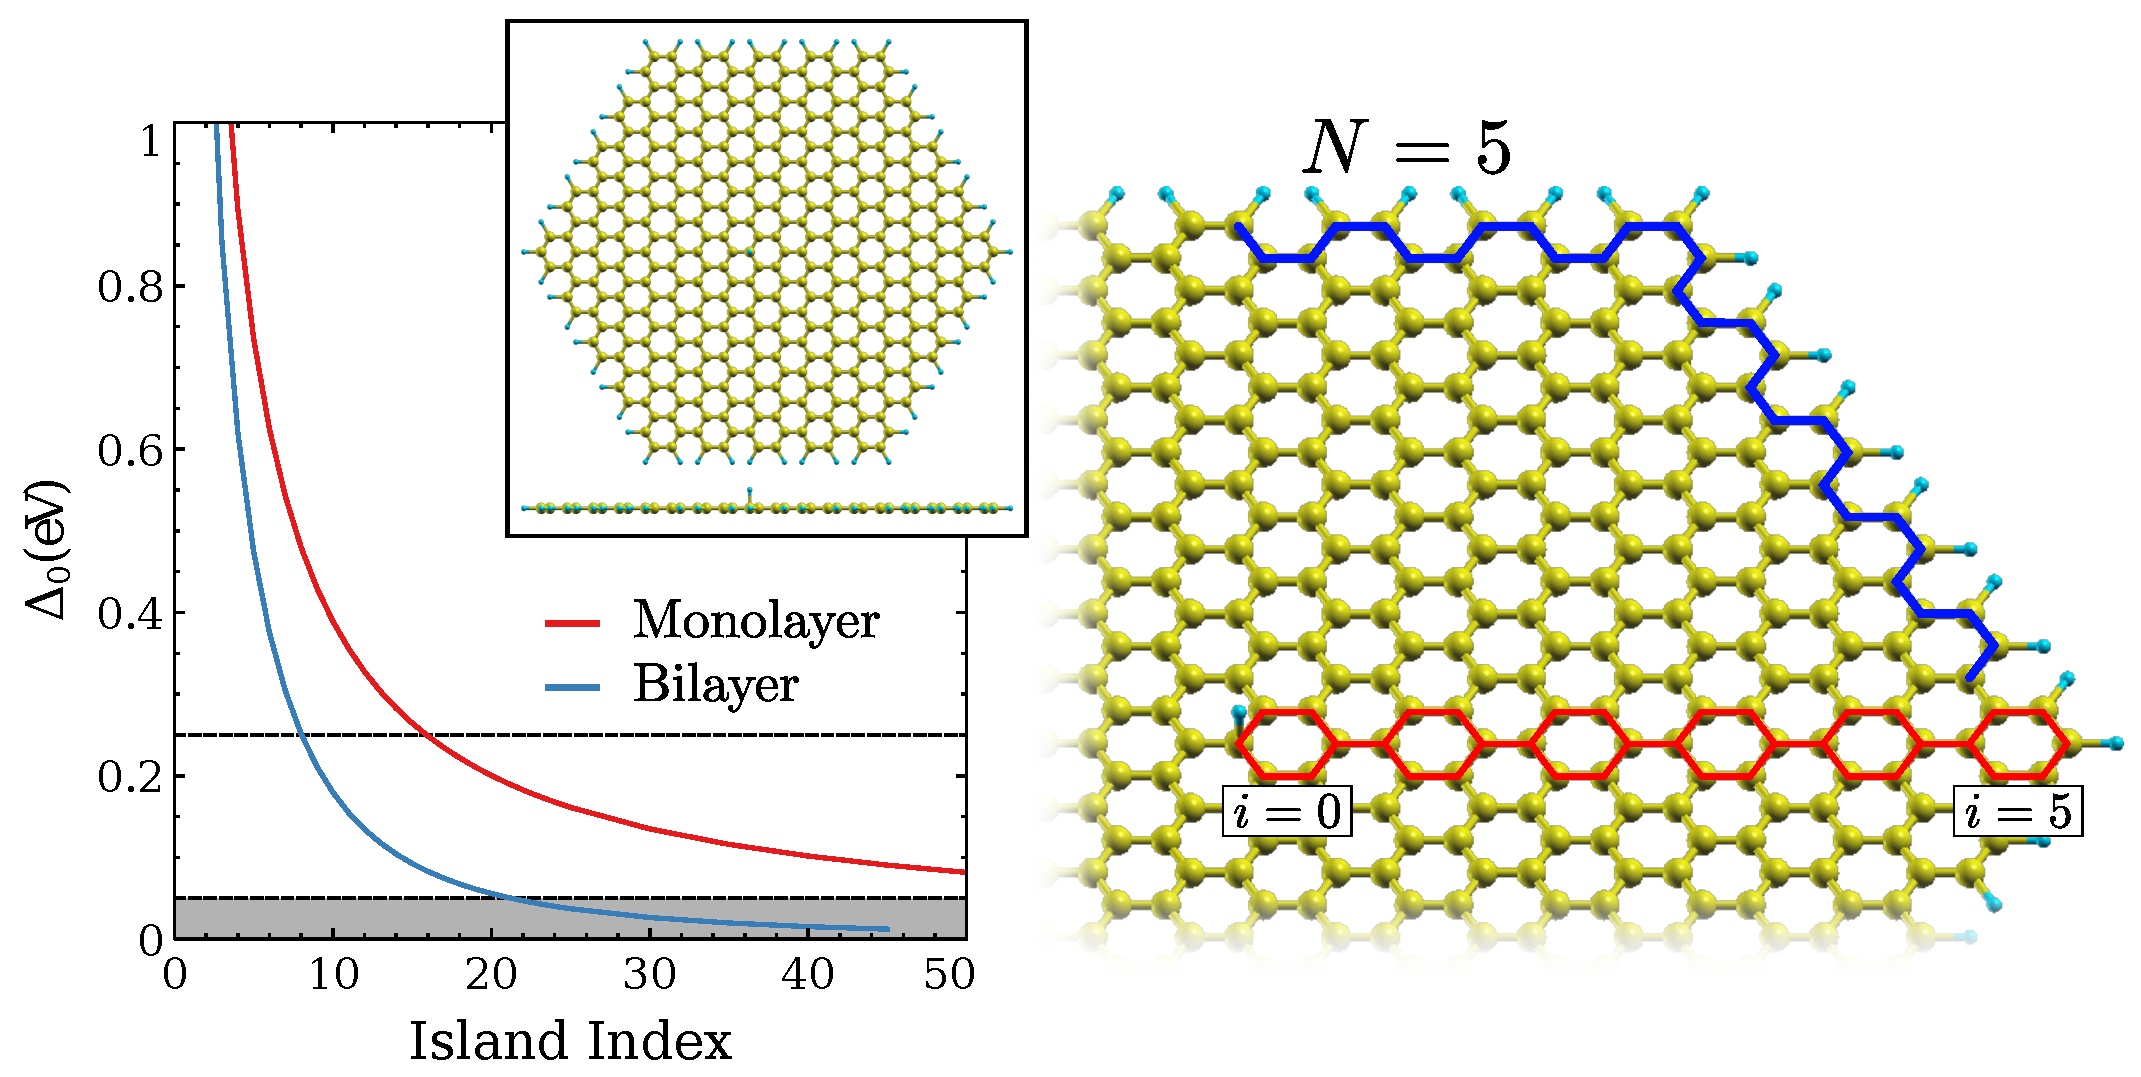
\includegraphics[width=0.9\textwidth]{graphene/figures/cell.pdf}
%  \vspace{-5pt}
%\caption{Confinement gap for a monolayer and a bilayer of graphene. The island index labels the size of the island by the number of ``benzene blocks'' along the diagonal as shown in red in the right panel. The dashed line at $0.25eV$ corresponds to the largest gap opened bia electric gating in graphene bilayer\cite{Zhang2009}. We will consider the islands big enough to be considered as graphene when their confinement gap lies in the shadowed region.}
%\label{confinement}
%\end{figure}
%\FloatBarrier
%%~~~~~~~~~~~~~~~~~~~~~~~~~~~~~~~~~~~~~~~~~~~~~~~~~~~~~~~~~~~%
%
%When 4 orbitals are considered, the breaking of the $C_3$ symmetry at the edges (ie, the $C$ atoms in the edges are missing 1 neighbor) results in near-zero energy states due to the unmet $\sigma$ bonds, combination of $s$, $p_x$ and $p_y$. In order to get rid of these artificious states we consider the island edges to be pasivated by Hydrogen atoms as shown in Fig.~\ref{confinement}. This way the dangling bonds hybridize and get lifted/drowned to the $\sigma$ manifolds.
%Although physically founded, the inclusion of $H$ pasivating atoms is somehow a technical construct to remove the dangling bonds from the low energy spectrum, hence, the strength of the $C-H$ bonds is not relevant and it should suffice to shift the $\sigma$ states far away from the low energy part of the spectrum.
%
%
%
%
%%The \ac{sk} parameters used for graphene are:
%%\begin{equation}
%%  V_{ss\sigma}= \SI{-7.76}{\eV} \quad;\quad
%%  V_{sp\sigma}= \SI{8.16}{\eV} \quad;\quad
%%  V_{pp\sigma}= \SI{7.48}{\eV} \quad;\quad
%%  V_{pp\pi}= \SI{-2.7}{\eV}
%%\label{sk_params}
%%\end{equation}
%
%
%
